\usepackage{graphicx}

\section{\textbf{Architecture Design \& Implementation}}

% 다음은 우리의 전체적인 디자인을 다이어그램으로 도식화한 것이다.


\subsection{\textbf{Overall architecture}} \\
% 우리의 디자인은 크게 두 단계로 나뉜다. 카메라로 사람의 얼굴이 감지되었을 때 실시간으로 face drooping을 검사하는 1단계, 1단계에서 의심스러운 정황이 나타나면 좀 더 정밀한 판단을 위해 인공지능 모델에 정확한 사진을 보내서 답을 얻는 2단계로 구성되어 있다. 이렇게 2-level로 검진 시스템을 구축한 이유는 다음과 같다. 첫째, 컴퓨팅 리소스를 낭비하지 않는다. 실시간으로 카메라의 장면을 인공지능 서버에 보내서 검증하기에는 많은 자원이 낭비된다. 또한, 사람이 집 안에서 생활하면 다양한 각도로 찍힐텐데 이런 상황에서 face-drooping으로 잘못 인식할 수 있다. 이런 오류에 컴퓨팅 리소스를 낭비하지 않기 위해 우선 1단계에선 정밀성은 떨어지더라도 라즈베리 파이에서 구동 가능한 정도의 검증 시스템을 구축해 얼굴의 비대칭 정도가 임계값을 넘을 때에만 2단계의 정밀 검증 시스템으로 넘어가도록 했다. 둘째, 개인정보를 보호할 수 있다. 집의 가구에 설치되는 카메라는 필연적으로 개인정보에 민감할 수 밖에 없다. 그래서 사진을 언제 촬영하는지 사용자에게 시각적으로 알려주는 방식을 생각했다. 애플의 맥북 같은 경우, 웹캠이 작동되면 언제나 초록색 불빛이 들어온다. 마찬가지로 우리의 시스템 역시 사진이 촬영될 때는 하드웨어적으로 불빛이 들어오도록 구현해 사생활 침해의 요소를 줄일 수 있다. 셋째, IoT 기기 의 성능을 고려했다. 가구에 탑재되는 IoT 기기는 성능이 충분하지 않다. 이런 기기에 너무 많은 기능을 한번에 탑재하면 전기가 많이 필요하고 이는 가구의 전기 효율은 낮추는 결과를 낳는다. 이를 방지하면서 추후 MLOps를 구축하는데는 인공지능 모델은 2단계로 구분하는 것이 더 낫다고 판단했다.

\begin{figure}[h]
    \centering
    \includegraphics[width=8.5cm]{images/무제.drawio.png}
    \caption{Overall Design of 2-Level}
\end{figure}

Our design is divided into two main steps. It consists of a first stage where the camera checks for face drooping in real-time a person's face is detected, and a second stage where the photo is sent to an artificial intelligence model for more precise details to get an answer since suspicious circumstances are omitted in the first stage. The reason for establishing this two-stage inspection system is as follows.

First, it doesn't waste computing resources. It wastes a lot of resources to send camera scenes to an artificial intelligence server for verification in real time. Additionally, if a person lives inside the house, they will be photographed from various angles, and in this situation, it can be mistaken for face-drooping. In order to avoid wasting computing resources on such errors, we first built a verification system that can be run on a Raspberry Pi even if the accuracy is low in the first stage, and moves to the second stage of precision verification system only when the degree of facial asymmetry exceeds the threshold.

Second, personal information can be protected. Cameras installed on home furniture are inevitably sensitive to personal information. So, I thought of a way to visually inform the user when a photo was taken. In the case of Apple's MacBook, a green light always comes on when the webcam is activated. Likewise, our system is also implemented in hardware to turn on lights when a photo is taken, thereby reducing the element of privacy infringement.

Third, the performance of IoT devices was considered. IoT devices mounted on furniture do not have sufficient performance. If these devices are equipped with too many functions at once, they require a lot of electricity, which results in lowering the electrical efficiency of the household. To prevent this and build MLOps in the future, we decided that it would be better to divide the artificial intelligence model into two stages.\\  

%%%%%%%%%%%%%%%%%%%%%%%%%%%%%%%%%%%%%%%%%%%%%%%
% 라즈베리파이 쓴 이유 조금 더 구체적으로 추가하기
% 1단계의 작동 방식을 간단하게 알아보자. 1단계에서는 비디오 스트림을 이용해 실시간으로 face drooping을 감지한다. face landmark를 이용하여 drooping을 판단하는 값이 임계값을 초과하게 되었을 시 알림을 보내며 2단계로 보낼 사진을 찍는다. 이후 저장된 사진을 2단계에 전송하게 된다.

Let's take a quick look at how Step 1 operates. In this step, real-time face drooping is detected using a video stream. If the calculated value for drooping, based on face landmarks, exceeds a set threshold, an alert is sent, and a photo for Step 2 is taken. This captured photo is then sent to Step 2.\\
The threshold is determined through \cite{mvalue}the examination of the positional relationship between the coordinates of the outer edges of both left and right lips and the midpoint beneath the lower lip. This methodology draws inspiration from the findings of precedent studies and has been configured accordingly. In Step 1 detection, this value is obtained using face landmarks. However, using the m-value of 0.16 as suggested by research resulted in overly sensitive reactions due to the characteristics of the video stream. Therefore, the value was adjusted to 0.2, and its reliable operation was empirically confirmed through multiple simulations.

\begin{equation} 
	m = \frac{y_2-y_1}{x_2-x_1}
\end{equation}

\begin{equation}
    threshold = |m_l - m_r|
\end{equation}

% 이 임계값은 왼쪽과 오른쪽 각 입술 끝 좌표와 아랫입술에서의 가운데 좌표와의 관계를 통해 구해지며 선행 논문의 결과를 참조해 설정하였다.(논문 레퍼런스 및 m value구하는 식 넣기). 1단계 detection에서는 이 값을 face landmark를 이용해 구한다. 다만, 연구 결과대로 m-value를 0.16으로 사용할 시 Video stream의 특성상 너무 예민하게 반응하는 문제가 있었다. 따라서 값을 0.2 수정하였고 신뢰도 있게 작동함을 여러 시뮬레이션을 통해 경험적으로 알 수 있었다.


% 2단계의 작동 방식을 간단하게 알아보자. 2단계에서는 라즈베리파이에서 전달 받은 이미지를 뇌졸중인지 아닌지로 정확하게 판단해야 한다. 이미지 분류 알고리즘을 훈련시키고 이를 검증하고 배포한다. 이 과정에서 훈련과 검증 단계는 더욱 low level적인 이야기이므로 생략한다. 배포 과정은 AWS의 AI 서비스 중 하나인 Amazon Rekognition이나 uvicorn을 사용한다. 이 중 Amazon Rekognition은 모델의 훈련, 검증, 배포를 한번에 진행할 수 있게 도와준다. uvicorn을 이용해서 웹 서버를 열어서 배포를 하는 경우, 입력은 이미지 파일을 받고 flatten시켜 모델의 입력값으로 넘겨준다. 반환값은 0 또는 1과 각각의 판단 확률값이다. 이때 반환값은 각각 no stroke, stroke이다. Amazon Rekognition을 이용했을 때의 입력은 똑같이 이미지 파일이다. 하지만 다른 점은 명시적으로 flatten시키지 않고 반환값은 string으로 'stroke_data' 혹은 'noStroke_data'와 각 판단의 Confidence 값이다.

Let’s take a quick look at how step 2 works. In the second step, the image received from the Raspberry Pi must be accurately judged as to whether it is a stroke or not. Train an image classification algorithm, verify it, and deploy it. In this process, the training and verification stages are omitted as they are more low-level. The deployment process uses Amazon Rekognition or uvicorn, one of AWS's AI services. Among these, Amazon Rekognition helps you train, verify, and deploy the model all at once.
When opening and distributing a web server using uvicorn, an image file is received as input, flattened, and passed as an input value to the model. The return value is 0 or 1 and the respective judgment probability value. At this time, the return values are no stroke and stroke, respectively. The input when using Amazon Rekognition is the same image file. However, the difference is that it is not explicitly flattened, and the return value is a string of 'stroke\_data' or 'noStroke\_data' and the confidence value of each judgment.\\

\begin{figure}[h]
    \centering
    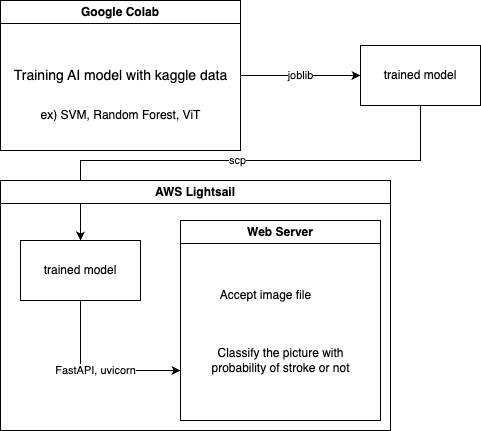
\includegraphics[width=8.5cm]{images/ai-back.drawio (1).png}
    \caption{Architecture when using no-AWS AI service}
\end{figure}


% MLOps를 위한 구현을 살펴보자. AWS를 사용한 이유는 추후의 확장성을 위해서이다. AWS Sagemaker를 이용하면 머신러닝 모델의 학습을 완전 자동화하거나 이미 존재하는 파편화된 코드들을 모아서 파이프라이닝 할 수 있다. 이런 작업을 거치면 ... 우리는 일회성으로 뇌졸중만 판단하는 시스템을 만들고 끝이 아니라 이를 바탕으로 더 거대한 하나의 생태계를 만들 수 있다. 그 기반에는 MLOps가 필수적이다. 데이터 과학자, 데이터 엔지니어, 직무 전문가, 머신러닝 아키텍트 전부 하나의 작업 환경 아래에서 작업할 수 있고, 자동화한다. 이를 바탕으로 다른 새로운 질병을 예측하는 머신러닝 기반 기기를 쉽게 제작하고, 훈련, 배포를 할 수 있다. 이런 생태계를 구축해 놓음으로써 의료, 건강 부분에서 머신러닝 기반 고객 관리 시스템을 쉽게 만들 수 있다.
Let's look at the implementation for MLOps. The reason for using AWS is for future scalability. Using AWS Sagemaker, you can completely automate the learning of machine learning models or pipeline existing fragmented codes. By going through this work... we can create a system that only judges strokes on a one-time basis and create a larger ecosystem based on this. MLOps is essential for that foundation. Data scientists, data engineers, job experts, and machine learning architects can all work under one work environment and automate it. Based on this, machine learning-based devices that predict other new diseases can be easily created, trained, and distributed. By establishing this ecosystem, it is possible to easily create a machine learning-based customer management system in the medical and health sectors.


\subsection{Directory structure}

\begin{table}[h]
\caption{Directory Structure}
\begin{tabular}{|p{4cm}|p{3cm}|p{2cm}|}
\hline
Directory & File names & Module names in use \\ \hline
/Raspberry/First\_level\_detection & first\_level.py & First\_level detection \\ \hline
/Raspberry/First\_level\_detection & detect\_face.py & First\_level detection\\ \hline
/Raspberry/First\_level\_detection & take\_photo.py & First\_level detection\\ \hline
/Raspberry/First\_level\_detection & image\_send.py & First\_level detection\\ \hline
/Raspberry/First\_level\_detection & count\_clock.py & First\_level detection\\ \hline
/Raspberry/First\_level\_detection & send\_aws.py & First\_level detection\\ \hline
/Raspberry/First\_level\_detection & voice\_alert.py & First\_level detection\\ \hline
model/AWS-Rekognition   &    classifier.py        &      AI-back  \\ \hline
model/Random-Forest   &  SE\_RandomForest.ipynb rf\_stroke\_classification       &   AI-back   \\ \hline
model/SVM   &     SE\_SVM.ipynb se\_svm.py      &          AI-back        \\ \hline
model/ViT   &      SE\_ViTprac.ipynb \newline se\_vitprac.py     &          AI-back \\ \hline
model/deployment & app.py & AI-back \\ \hline
\end{tabular}
\end{table}

\subsubsection{Module1: First\_level detection}
%1단계 detection은 face landmark를 이용한다. 이것은 Video stream을 이용해 실시간으로 정보를 처리하며, 뇌졸중의 징후인 mouth droop이 보일 때 사진을 찍어 2단계 모델로 전송한다. 1단계 detection은 징후가 조금이라도 포착되면 작동하기 때문에 정확도가 높지 않다. 신뢰도 있는 판정은 2단계에서 해주므로 1단계 detection의 의의는 real-time 처리 및 자원 사용의 효율성 및 개인 정보 보호로 볼 수 있을 것이다. 다만, IoT에 적용될 프로그램을 생각하면서 만들었기에 한정된 자원의 효율적 사용 또한 매우 중요한 지점이 될 것이다.
Step 1 detection relies on face landmarks, processing real-time information through a video stream. It takes a photo when it detects signs of mouth drooping, indicative of a stroke, and sends it to the Step 2 model. Since Step 1 activates upon detecting even slight indications, its accuracy may not be very high. The significance of Step 1 detection lies in its real-time processing, efficient use of resources, and privacy protection. However, given its design for application in IoT programs, the efficient use of limited resources is also a critical consideration.\\


\begin{figure}[h]
    \centering
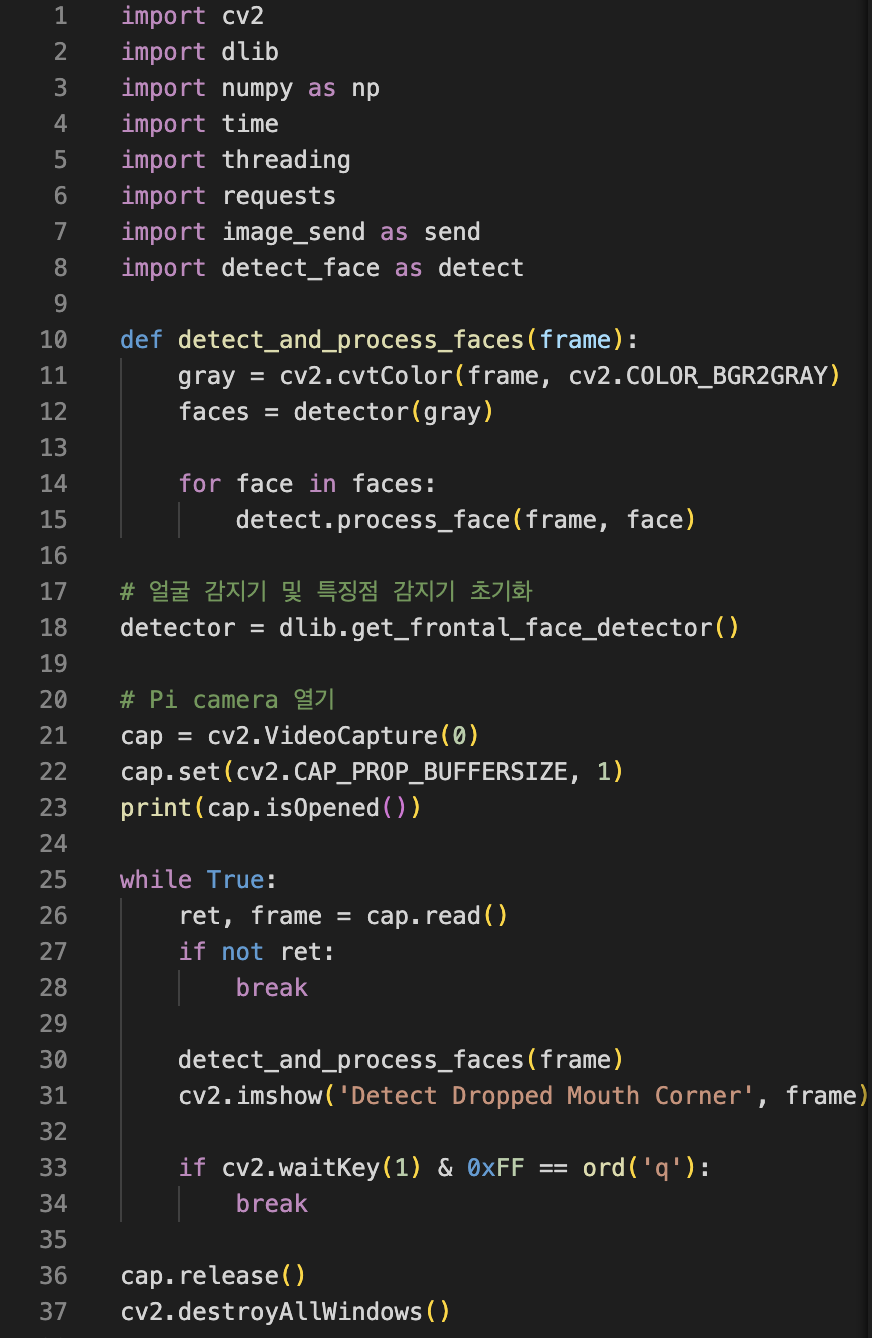
\includegraphics[width=0.5\linewidth]{images/first_level.png}
    \caption{first\_level.py}
    \label{fig:enter-label}
\end{figure}

\textbf{first\_level.py}
% main이 되는 실행파일로 OpenCV 라이브러리를 통해 camera로 부터 Video Stream 정보를 가져온다. 라즈베리파이의 하드웨어적 한계로 인해 Buffer size를 최소화여 Video Stream를 불러와야 한다. 이후 cv2.imshow를 통해 처리된 video stream을 볼 수 있다. 또한 first_level.py에서 처리되는 정보를 Gray scale로 변경해준다. Gray Scale을 사용하는 이유는 첫 째, 정보의 용량이 감소한다. RGB를 사용할 경우 RGB 3개의 색상 channel이 생기므로 처리할 정보가 늘어난다. 본 프로젝트에서는 색상 정보가 필요하지 않기때문에 gray scale로 변경해 용량을 줄이고 처리 속도를 향상시키고자 하였다. 둘 째, 노이즈가 감소한다. IoT 장비에 들어가는 카메라는 고성능일 수 없다. 따라서 화질이 안좋은 만큼 노이즈가 많을텐데 gray scale로 변경함으로써 노이즈를 줄이고 우리가 원하는 drooping 정보를 깔끔하게 얻을 수 있다. gray scale로 변경하는 작업은 픽셀을 하나씩 변경해주어야하는데 OpenCV에서 cv2.cvtColor 함수를 제공하기에 이를 사용해서 simple하게 바꿀 수 있다. 또한 face landmark 탐지를 위해 dlib 함수를 사용해 gray scale로 변경된 Video stream을 이 함수에 전달해주는 것까지 해당 파일에서 진행한다.

The main executable file uses the OpenCV library to capture video stream information from the camera. Due to hardware limitations of the Raspberry Pi, it is essential to minimize the buffer size for loading the video stream. Subsequently, the processed video stream can be viewed using cv2.imshow. Additionally, the information processed in first\_level.py is converted to grayscale. The rationale behind using grayscale is twofold. Firstly, it reduces the data size since using RGB would introduce three color channels, increasing the processing load. As color information is unnecessary for this project, converting to grayscale reduces the data size, enhancing processing speed. Secondly, it decreases noise. Cameras for IoT devices may not be high-performance, resulting in potentially noisy images. Converting to grayscale helps mitigate noise, allowing us to obtain clean drooping information. The task of converting to grayscale involves altering each pixel, a task facilitated by the cv2.cvtColor function in OpenCV. Furthermore, in the same file, the video stream, now in grayscale, is passed to the dlib function for face landmark detection.\\

\begin{figure}[h]
    \centering
    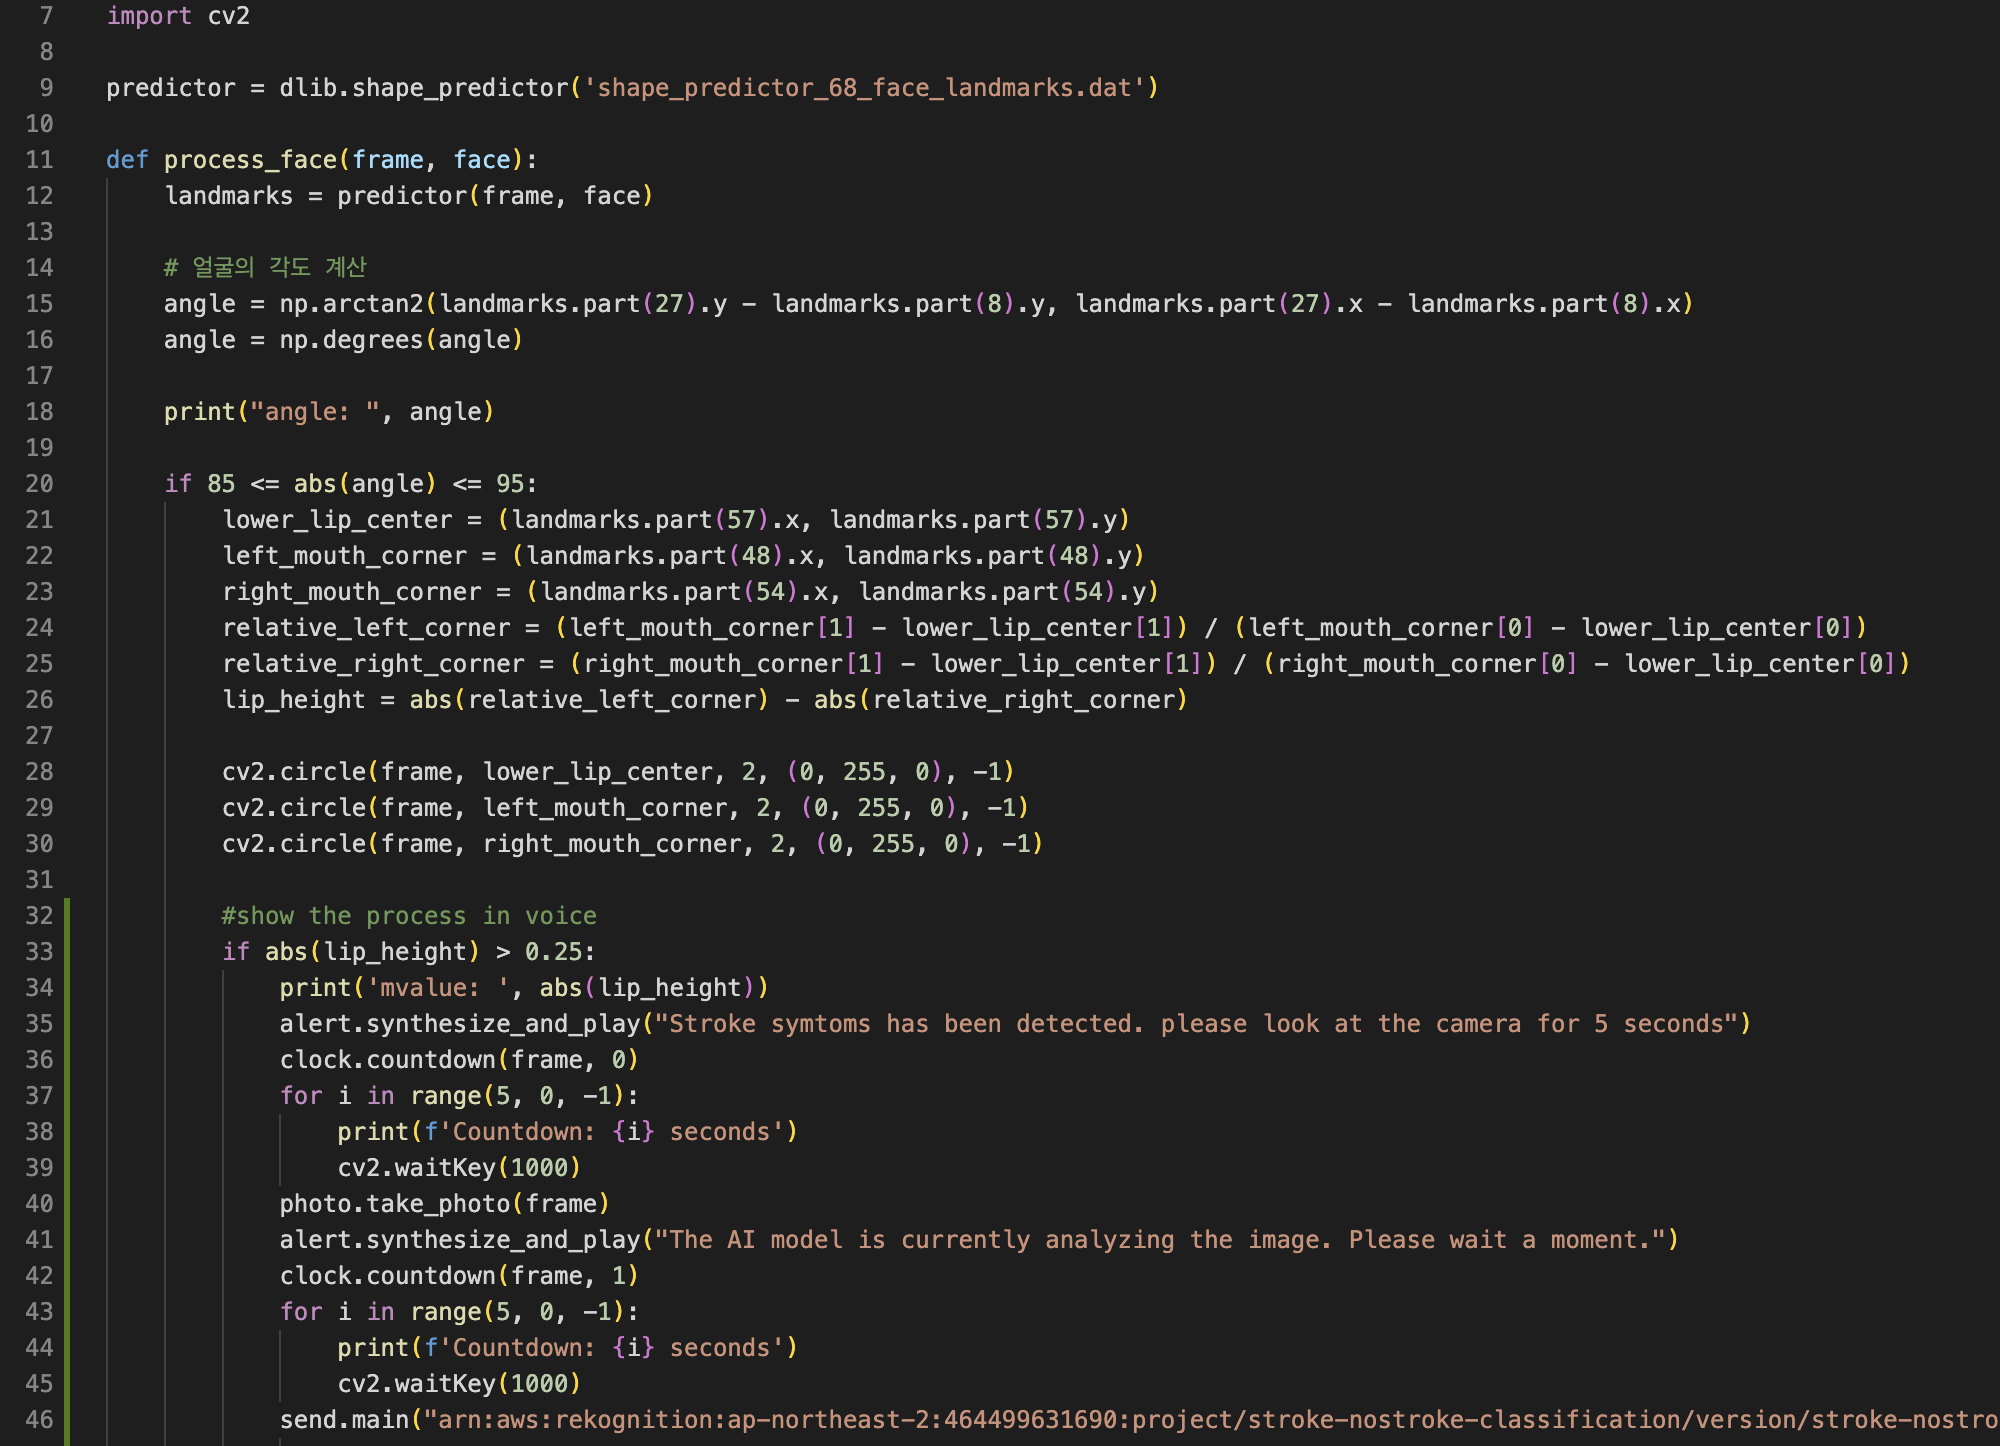
\includegraphics[width=0.5\linewidth]{images/detect_face.png}
    \caption{detect\_face.py}
    \label{fig:enter-label}
\end{figure}

\textbf{detect\_face.py}
%detect_face에서는 m-value를 계산하여 first detection을 수행한다. 또한 Video Stream을 처리하기 때문에 과하게 얼굴 각도가 기울어져있으면 결과에 영향을 주기도 한다. 그래서 먼저 얼굴 각도를 계산한다. landmark의 27번 인덱스와 8번 인덱스는 얼굴의 상하단 좌표이다. numpy의 arctan함수를 사용해 각도를 구하고 이 각도가 85도에서 95도 사이일 경우에만 first_level detection이 진행된다. 이후 m-value를 구한다. landmark의 57번 인덱스는 아랫입술의 가운데 좌표이고, 48번은 왼쪽 끝, 54번은 오른쪽 끝 좌표이다. 아랫입술과 양쪽 입술 끝의 차이를 relative_corner로 구하며 이 차이가 곧 m_value가 된다. 이 m_value가 0.25 이상일 경우에 first_level detection에 잡히게 되고 이후 second_level detection을 위한 사진을 촬영한다. 동시에 이를 aws polly를 이용해 voice로 알림을 준다. 추가로 frame에서의 입술의 좌표를 보여주는 것과 face landmark를 위한 dlib의 보조 파일을 주는 것까지 detect_face.py에서 수행한다.

In the detect\_face module, the m\_value is computed to perform the initial detection. Given that it processes a video stream, excessively tilted face angles can impact the results. Therefore, the first step involves calculating the face angle. Landmark indices 27 and 8 represent the top and bottom coordinates of the face. Using the arctan function of numpy, the angle is computed, and first-level detection proceeds only when this angle between 85 and 95 degrees. After that, the m-value is determined. Landmark index 57 corresponds to the center coordinate of the lower lip, while 48 and 54 represent the left and right ends, respectively. The difference between the lower lip and the ends of both lips, known as relative\_corner, becomes the m-value. If this m\_value is greater than or equal to 0.25, it triggers the first-level detection, capturing a photo for subsequent second\_level detection. Simultaneously, an alert is provided using AWS Polly in a voice format. Additionally, detect\_face.py handles displaying lip coordinates on the frame and providing auxiliary files for face landmarks using dlib.\\

\begin{figure}[h]
    \centering
    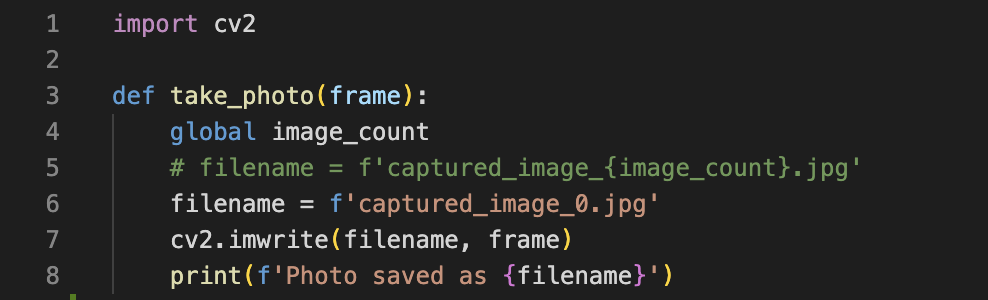
\includegraphics[width=0.5\linewidth]{images/take_photo.png}
    \caption{take\_photo.py}
    \label{fig:enter-label}
\end{figure}

\textbf{take\_photo.py}
%take_photo.py는 second_level detection으로 전송할 사진을 찍는 기능을 수행한다. openCV의 imwrite 함수를 활용해 현재 frame에 잡혀있는 모습을 이미지로 저장한다. IoT에 들어갈 소프트웨어이기 때문에 찍은 사진을 전부 저장하지 않고 가장 최근에 찍은 사진만을 local에 저장한다. 이전 이미지들은 second_level로 전송됨과 동시에 aws cloud에 저장된다. 

The take\_photo.py module serves the functionality of capturing a photo to be sent for second-level detection. It utilizes the imwrite function from OpenCV to save the current frame as an image. Given its purpose as software for IoT, it only retains the most recently captured photo locally, instead of storing all the taken pictures. Previous images are sent for second\_level detection and concurrently stored in the AWS Cloud.\\

\begin{figure}[h]
    \centering
    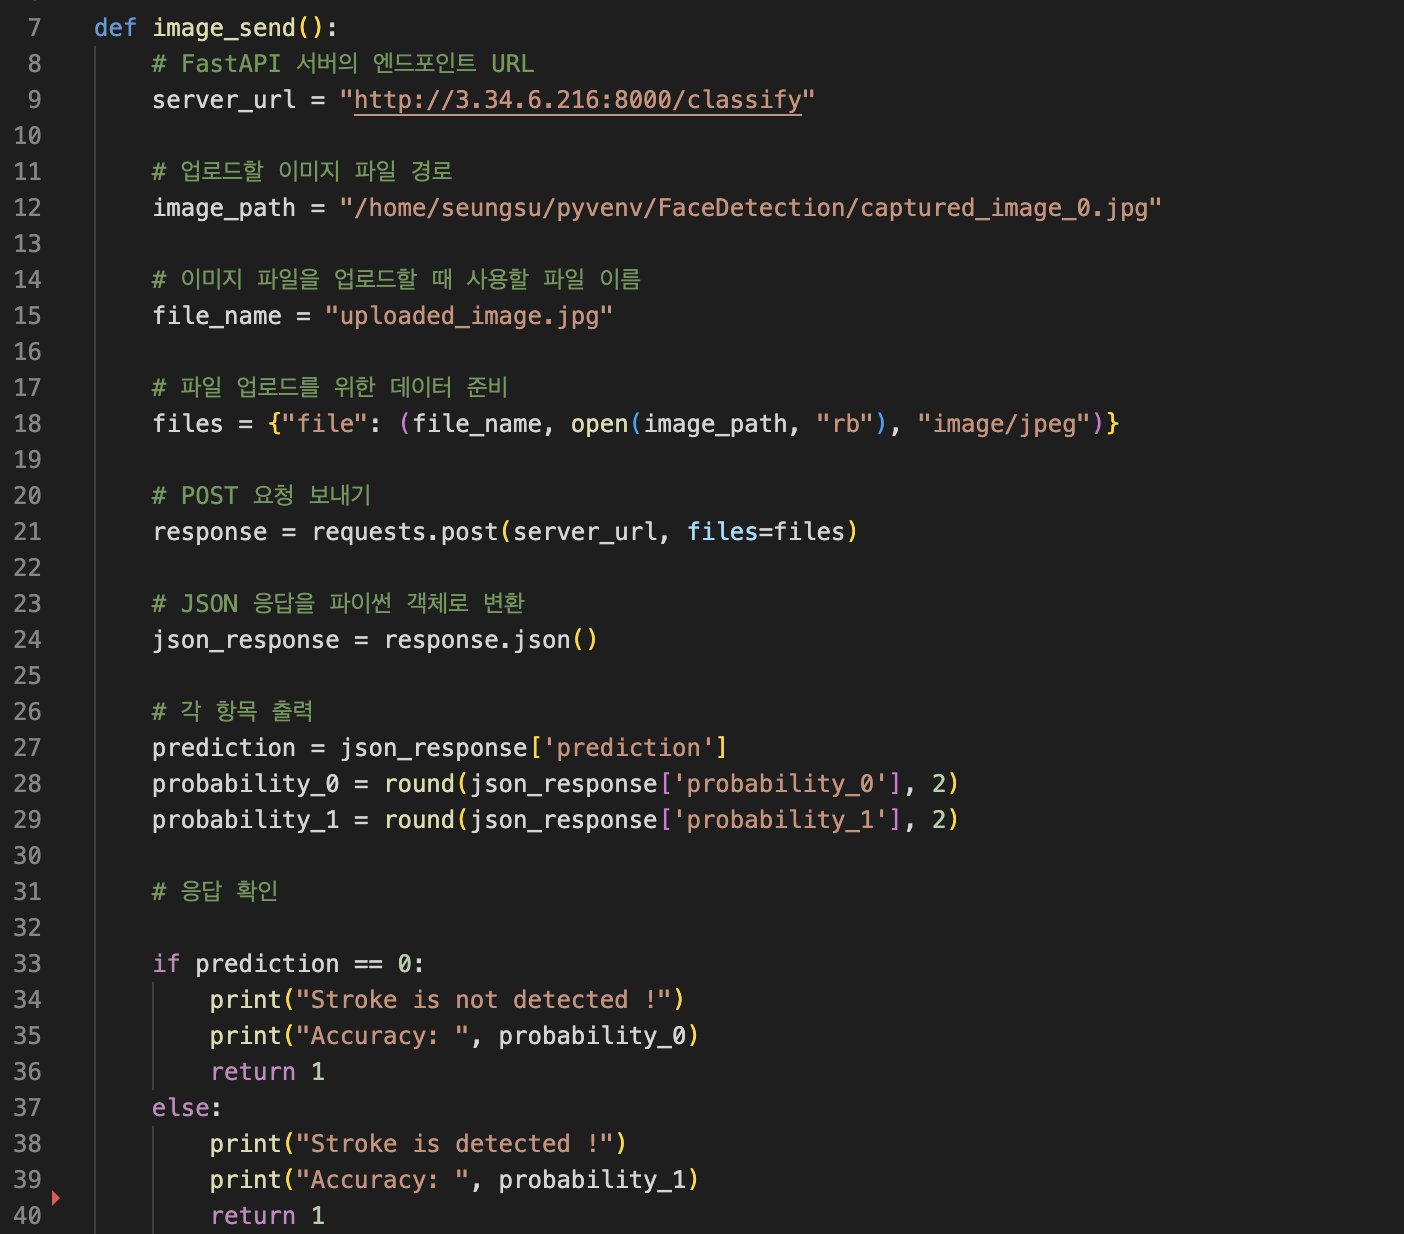
\includegraphics[width=0.5\linewidth]{images/image_send.png}
    \caption{image\_send.py}
    \label{fig:enter-label}
\end{figure}

\textbf{image\_send.py}
%image_send.py는 웹서버를 통해 second_level detection을 진행할 때 사용된다. 실행중인 웹서버의 url을 가지고 특정 이미지 파일을 전송한다. POST방식을 사용해 request를 보내고 json 파일로 response를 받는다. 이후 response된 json파일을 python 객체로 변환한 후 response의 인덱스에 따른 결과값을 확인한다. prediction이 0이라면 stroke이 탐지되지 않은 것이고 이외의 값이라면 탐지된 것이다. 이때 second_level model이 판단한 Accuracy까지 user에게 보여준다.

The image\_send.py module is used when going second-level detection through a web server. It sends a specific image file to the running web server's URL using the POST method, then receives the response in the form of a JSON. Subsequently, it converts the received JSON file into a Python object and checks the result based on the response index. If the prediction is 0, it indicates that a stroke has not been detected; otherwise, it signifies a detection. Additionally, it displays the accuracy determined by the second-level model to the user.\\

\begin{figure}[h]
    \centering
    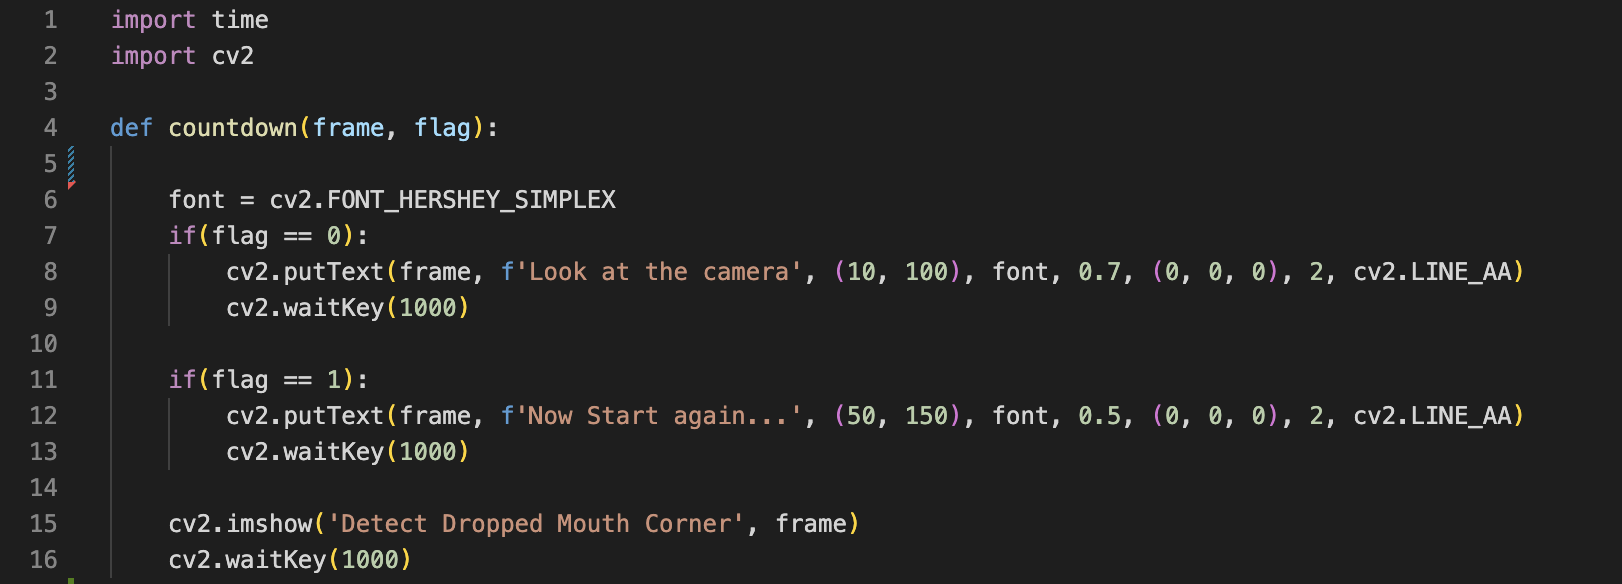
\includegraphics[width=0.5\linewidth]{images/count_clock.png}
    \caption{count\_clock.py}
    \label{fig:enter-label}
\end{figure}

\textbf{count\_clock.py}
%count\_clock.py는 openCV imshow frame에 카운트를 띄우는 기능을 한다. first_level에서 Mouse drooping이 발견되면 사진을 찍기 전 "Look at the camera"를, 사진을 찍은 후엔 다시 first_level로 돌아가기 전까지 "Now Start again..."을 보여준다.

The count\_clock.py module performs the function of displaying a count on the OpenCV imshow frame. When Mouse drooping is detected in the first\_level, it shows "Look at the camera" before taking a photo, and after capturing the photo, it displays "Now Start again..." until returning to the first\_level.\\

\begin{figure}[h]
  \centering
  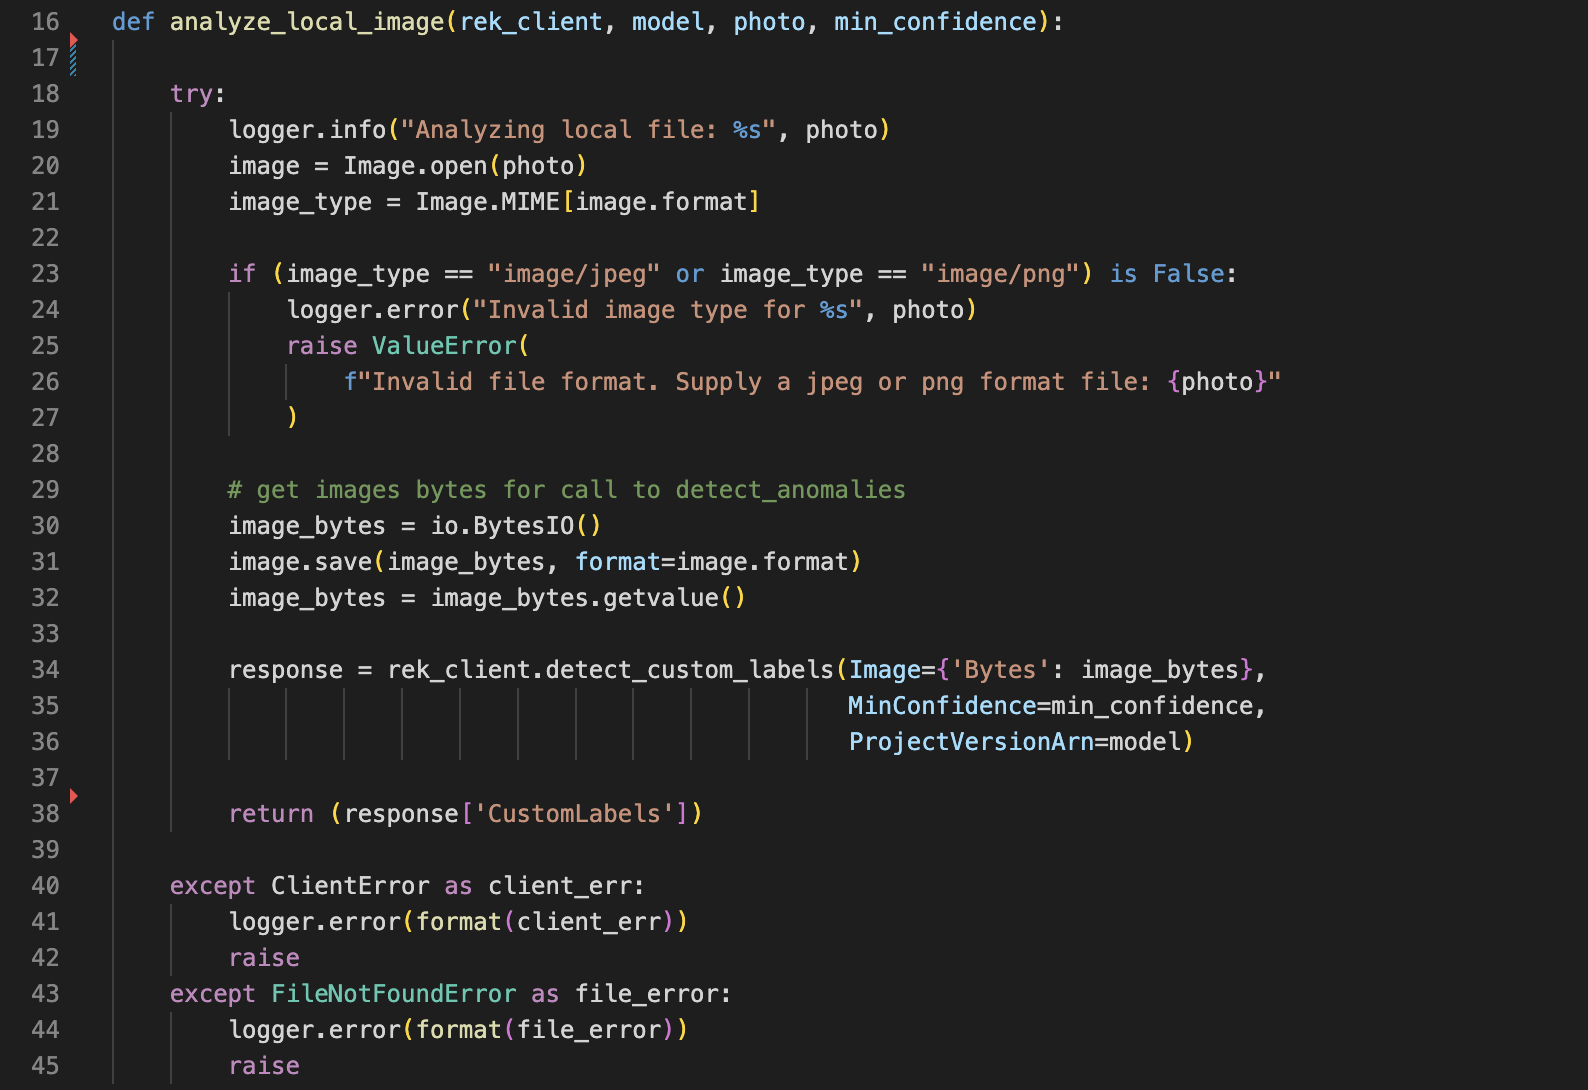
\includegraphics[width=0.45\textwidth]{images/send_aws_1.png}
  \hspace{0.05\textwidth}
  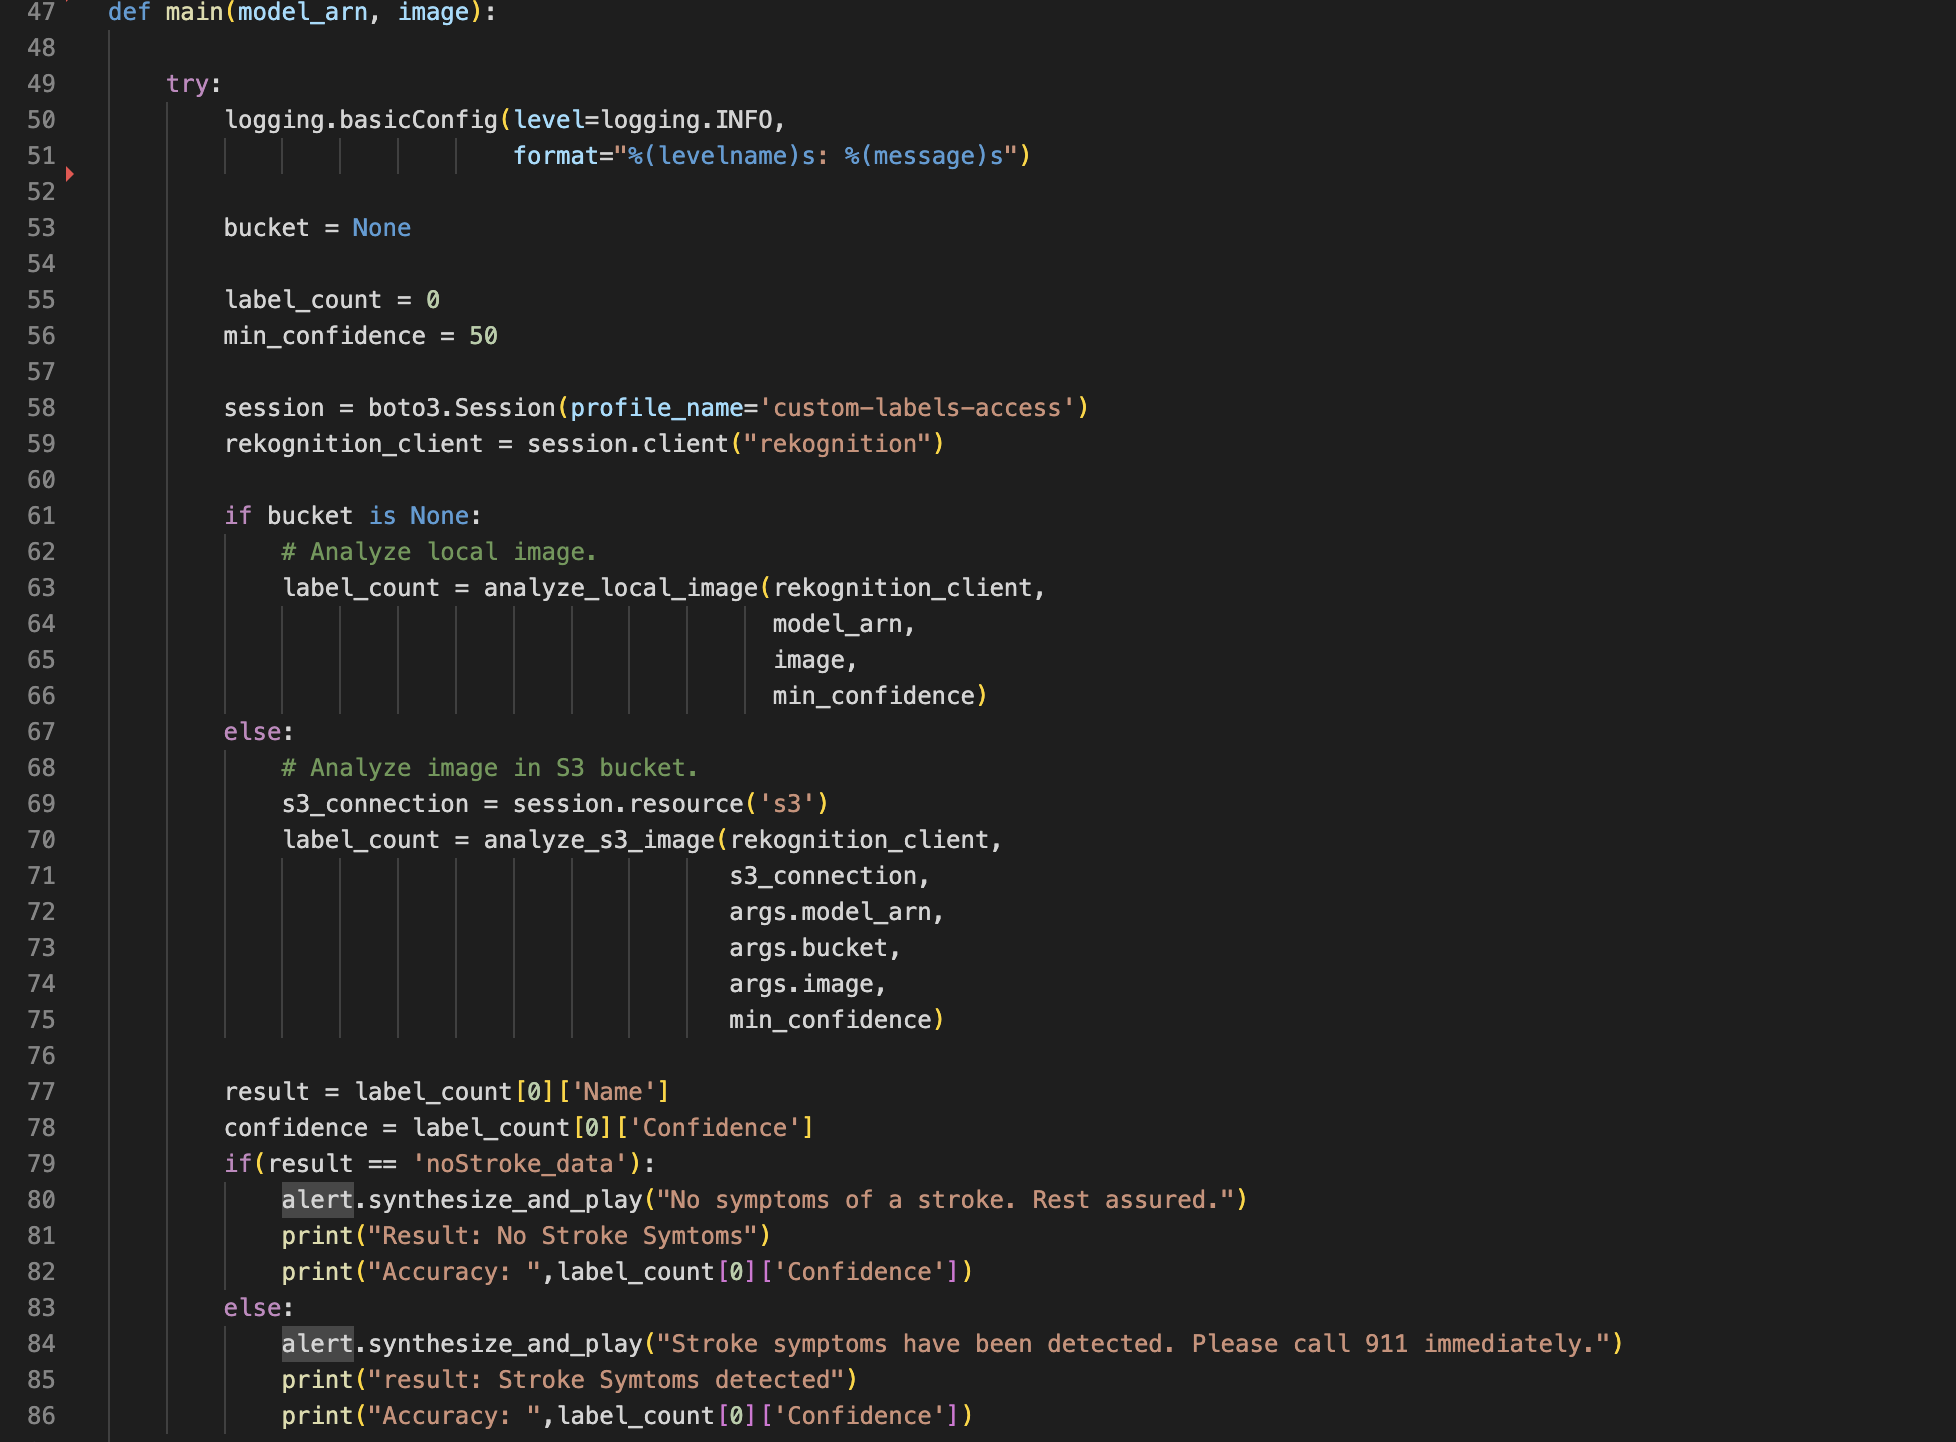
\includegraphics[width=0.45\textwidth]{images/send_aws_2.png}
  \caption{send\_aws.py}
  \label{fig:twopics}
\end{figure}

\textbf{send\_aws.py}
This script utilizes the AWS Rekognition service to detect custom labels in images and generate voice alerts based on the detected labels. The code reads an image from a local file, uses the Amazon Rekognition Custom Labels to detect labels defined in a custom model, and triggers voice alerts accordingly.

Key functions and components:
\begin{enumerate}
    \item analyze\_local\_image: 
    This function reads an image from a local file, uses Amazon Rekognition Custom Labels to detect labels in the user-defined model, and returns the detected labels.\\
    \item main: 
    The main function of the script takes the model ARN and image path as input, analyzes the image, and generates a voice alert based on the results.\\
    \item The code interacts with AWS services using the Boto3 AWS SDK. It sets up a session with boto3.Session and communicates with the Rekognition service through the rekognition\_client.
    \item Voice alerts are generated using the voice\_alert module, specifically the synthesize\_and\_play function, which synthesizes text into speech and plays it.\\
    \item Error handling is implemented to appropriately handle exceptions, and logging is used to output information and error messages.\\
    \item The section if \_\_name\_\_ == "\_\_main\_\_": is the typical entry point for a Python script, ensuring that the main function is called only when the script is executed directly.\\
\end{enumerate}
This code primarily focuses on utilizing the AWS Rekognition service for image processing and custom label detection, demonstrating the functionality of an application that triggers voice alerts based on image analysis results.\\

\begin{figure}[h]
  \centering
  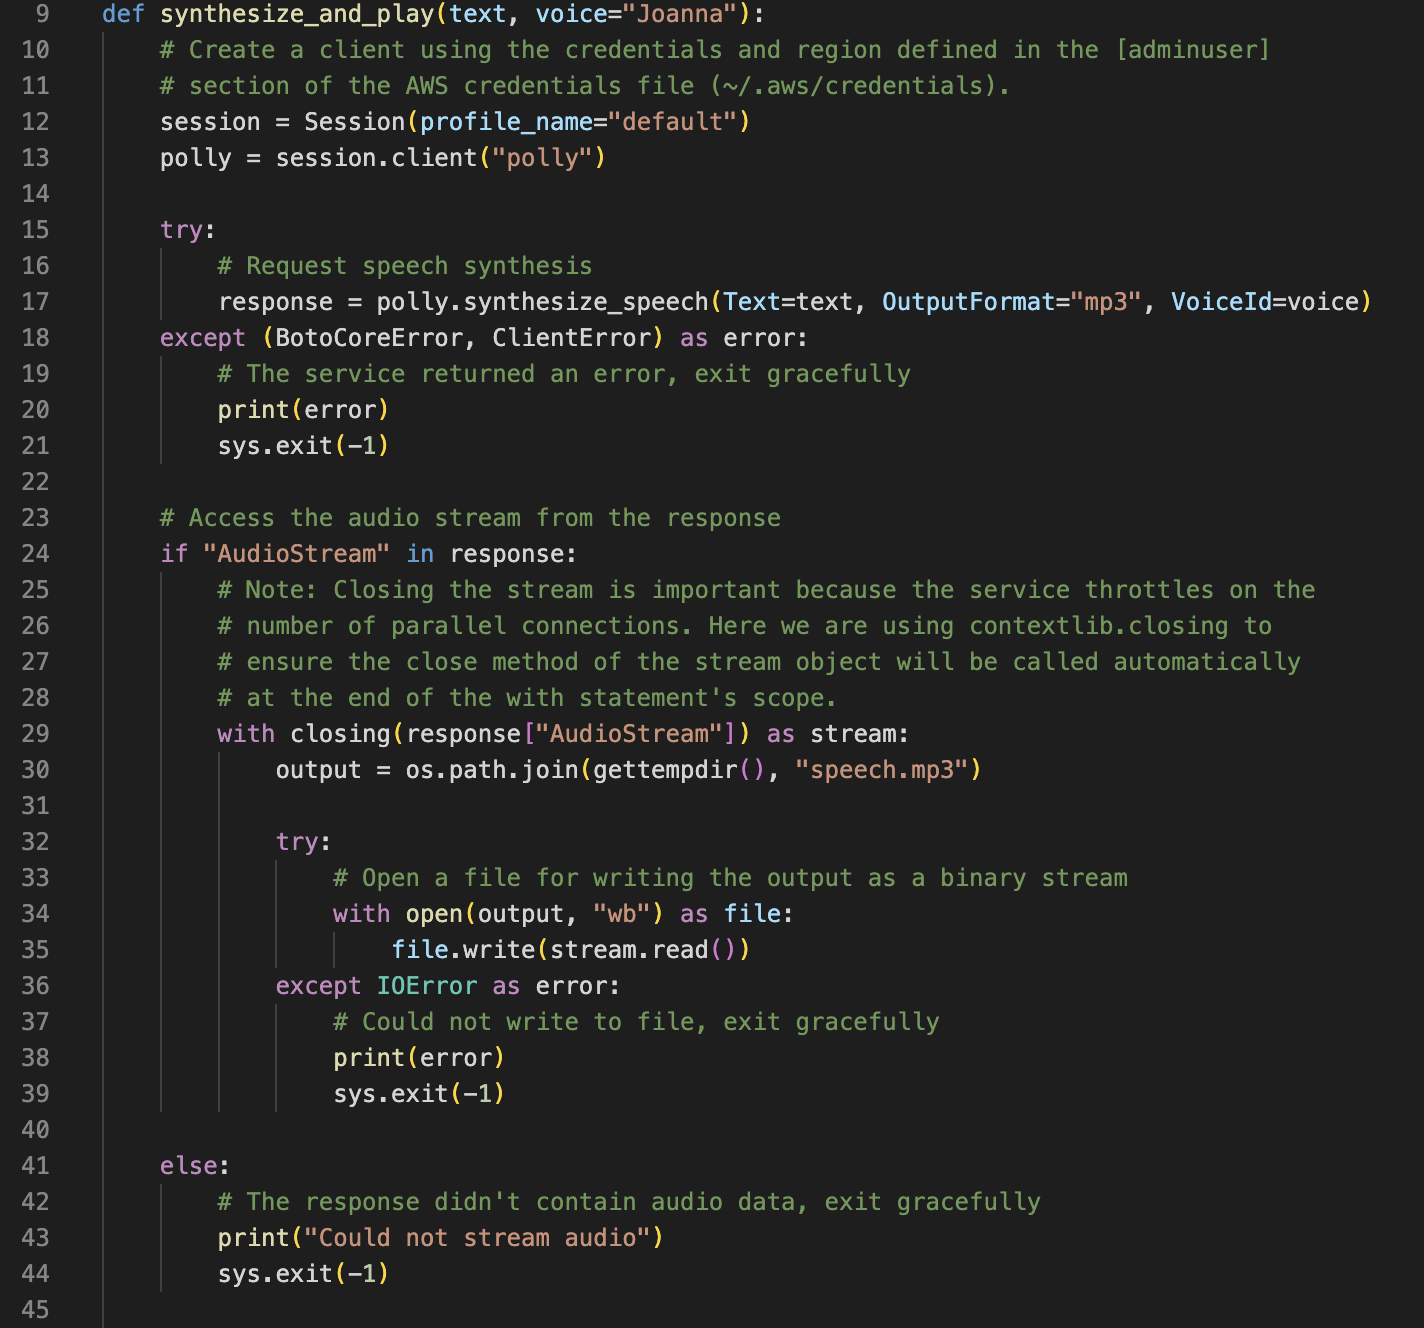
\includegraphics[width=0.45\textwidth]{images/voice_alert_1.png}
  \hspace{0.05\textwidth}
  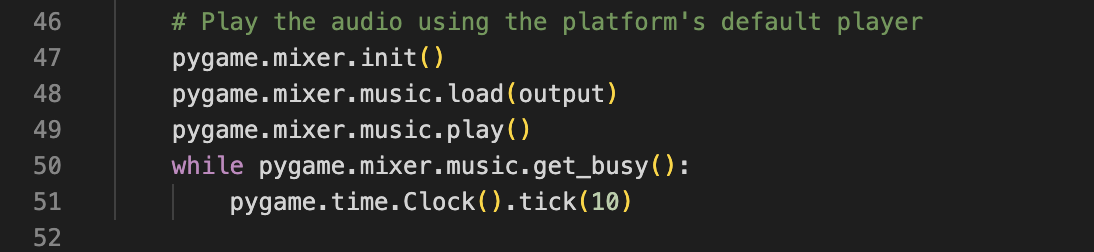
\includegraphics[width=0.45\textwidth]{images/voice_alert_2.png}
  \caption{alert\_aws.py}
  \label{fig:twopics}
\end{figure}

\textbf{voice\_alert.py}
This is designed to synthesize speech from a given text using the Amazon Polly service and play the resulting audio.

\begin{enumerate}
    \item Input Parameters:
    text: The input text that needs to be synthesized into speech.
    voice (optional, default is "Joanna"): The voice to be used for speech synthesis.
    \item Function Steps:
    It creates an AWS Polly client using the AWS credentials and region defined in the [default] section of the AWS credentials file (~/.aws/credentials).
    Attempts to synthesize speech by making a request to Polly with the provided text, specifying the desired output format ("mp3") and voice.
    Handles potential errors such as BotoCoreError or ClientError that may occur during the Polly service request. If an error occurs, it prints the error message and exits the script with an error code (-1).
    If the response from Polly contains an audio stream ("AudioStream"), it saves the audio stream to a temporary mp3 file on the local system.
    If there is an issue with streaming audio or writing to a file, it exits gracefully, printing an error message.
    Finally, it uses the Pygame library to play the synthesized speech using the platform's default audio player. It ensures that the program doesn't exit until the audio has finished playing.
    \item Dependencies:
    The function depends on the boto3 library for AWS interaction and the pygame library for audio playback.
    \item Note:
    Make sure to have the necessary AWS credentials configured on the system.
\end{enumerate}

The script expects Pygame to be installed for audio playback.
Overall, this function provides a convenient way to synthesize speech from text using Amazon Polly and play the generated audio using the Pygame library.

\begin{figure}[h]
    \centering
    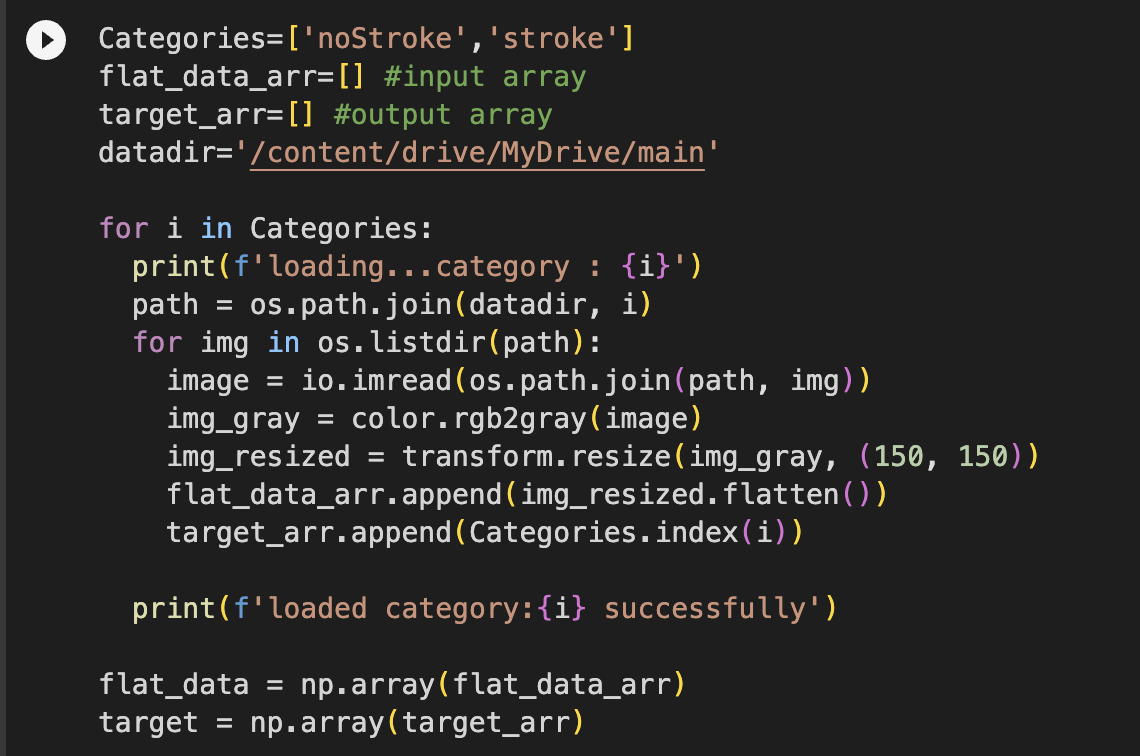
\includegraphics[width=8.5cm]{images/rf_data.png}
    \caption{Pre-processing data in Random Forest}
    \label{fig:enter-label}
\end{figure}

\subsubsection{Module2: AI-back}
% AI-back 모듈은 2-Level detection에서 2단계를 구성하는 요소이다. 인공지능 모델로 3가지를 생각했다. 머신러닝 기반의 Support Vector Machine과 앙상블 학습을 하는 Random Forest, 그리고 딥러닝 기반의 ViT를 각각 만들고 실험했다. ipynb 파일은 Google Colab에서 작성한 코드이다.
The AI-back module is an element that constitutes the second stage in 2-Level detection. We thought of three things as an artificial intelligence model. We created and tested machine learning based Support Vector Machine, random forest using ensemble learning, and deep learning-based ViT. The ipynb file is code written in Google Colab.

\textbf{SE\_RandomForest.ipynb} \\
% Random Forest 머신러닝 모델을 사용하고 그 모델을 훈련시키는 노트북 파일이다. 파일은 크게 3부분으로 나뉜다. 첫째, 뇌졸중 환자와 정상인의 얼굴 데이터를 불러와서 전처리를 하는 과정. 둘째, 전처리한 데이터를 랜덤 포레스트 모델을 불러와서 학습시키는 과정. 마지막으로 훈련을 마친 모델을 테스트하는 과정이다.
This is a notebook file that uses the Random Forest machine learning model and trains the model. The file is divided into three parts. First, the process of loading and pre-processing face data of stroke patients and normal people. Second, the process of loading and training the random forest model on the preprocessed data. Lastly, it is the process of testing the trained model.

% 데이터 전처리는 다음과 같은 과정으로 이루어진다. 이미지를 폴더에서 불러오고 흑백으로 전환한다. 이미지의 색깔과 표정은 독립적이므로 입력의 차원값을 줄이는 방향으로 진행했다. 이미지 데이터의 크기가 제각각이므로 (150, 150)의 크기로 변환하고 이를 평면화해서 벡터로 만들었다. 
Data preprocessing consists of the following processes. Load an image from a folder and convert it to black and white. Since the color and expression of the image are independent, we proceeded to reduce the dimension of the input. Since the size of the image data is different, we converted it to a size of (150, 150) and flattened it into a vector.

\begin{figure}[h]
    \centering
    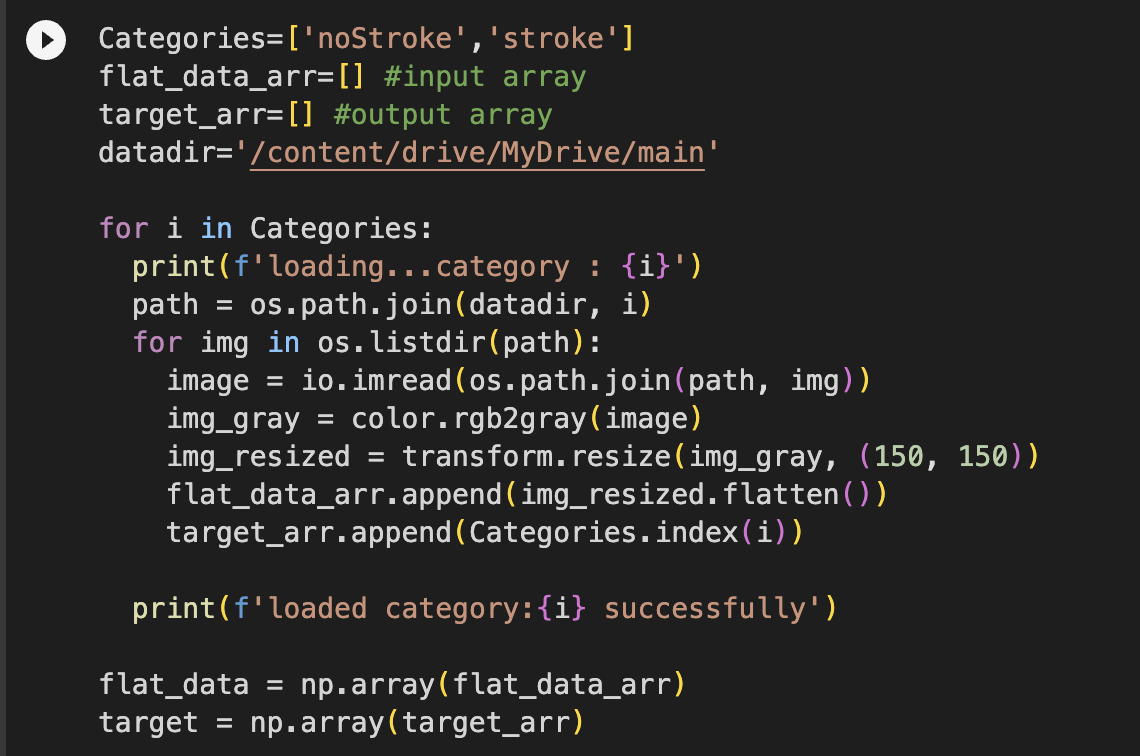
\includegraphics[width=8.5cm]{images/rf_data.png}
    \caption{Pre-processing data in Random Forest}
    \label{fig:enter-label}
\end{figure}

% 사이킷런의 라이브러리를 활용해 모델을 import했다. 훈련용 데이터와 테스트용 데이터를 80%, 20%로 나누고 훈련용 데이터로 학습시켰다. 이 과정은 수분밖에 소요되지 않았다.
The model was imported using scikit-learn’s library. The training data and testing data were divided into 80\% and 20\% and learned using the training data. This process took only a few minutes.

% 마지막으로 학습이 완료된 모델을 테스트 데이터로 검증한다. 이때, 단순한 정확도로는 뇌졸중 판단 모델의 성능을 확실시 할 수 없다. 사람의 건강을 판단하는 것이기 때문에 true positive, false negative 등 자세하게 판단해야 한다. classification_report 함수를 사용해서 더 정확한 성능을 판단한다.
Finally, the trained model is verified with test data. At this time, the performance of the stroke judgment model cannot be assured with simple accuracy. Since it is a judgment of a person's health, it must be judged in detail, including true positives and false negatives. Use the classification\_report function to determine more accurate performance.

% 아래는 실제 classification_report 함수를 적용한 결과이다. 주목해야 할 점은 stroke의 precision 값이 0.97로 매우 높다는 점이다. 이는 모델이 stroke라 판단했으면 실제로 stroke인 확률이 97%인 것이다. 반면 stroke recall은 0.72로 떨어지는데 이는 실제로는 stroke이지만 stroke로 모델이 판단을 하지 못한 것이 28%라는 뜻이다. 전체적으로 stroke의 정확도가 no-stroke 판단의 정화도보다 낮은데 이는 데이터의 갯수가 no-stroke가 많기 때문이라고 사료된다.
Below is the result of applying the actual classification\_report function. What is important to note is that the stroke precision value is very high at 0.97. This means that if the model determines that it is a stroke, there is a 97\% probability that it is actually a stroke. On the other hand, stroke recall drops to 0.72, which means that 28\% of cases were actually strokes, but the model failed to judge them as strokes. Overall, the accuracy of stroke is lower than the precision of no-stroke judgment, which is believed to be because the number of data is large.
\begin{figure}[h]
    \centering
    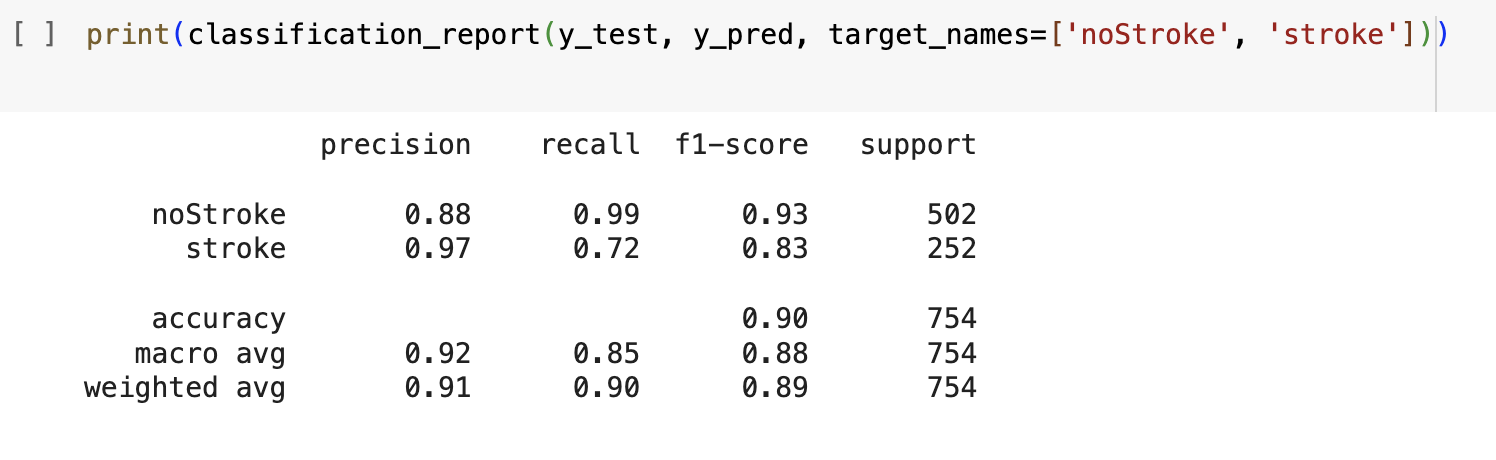
\includegraphics[width=8.5cm]{images/rf_result.png}
    \caption{The result of testing Random Forest model}
    \label{fig:enter-label}
\end{figure}


\textbf{rf\_stroke\_classification} \\
% 위의 파일로 훈련이 완료된 모델이다. joblib 함수로 파일을 저장했다. 이후 이 파일을 AWS Lightsail에 옮기고 후술될 app.py 파일에서 호출해서 웹 서버로 올린다. 이것으로 모델을 웹 서버로 배포한다.
This is a model that has been trained with the file above. The file was saved using the joblib function. Afterwards, move this file to AWS Lightsail and upload it to the web server by calling it from the app.py file, which will be described later. This deploys the model to the web server.

\textbf{SE\_SVM.ipynb} \\
% Support Vector Machine 기반으로 학습을 진행하는데 사용된 파일이다. Google Colab에서 작동했으며 SE\_RandomForest.ipynb 파일과 동일한 과정을 거쳐 데이터 전처리, 학습, 검증을 했다.
This is a file used to conduct learning based on Support Vector Machine. It ran in Google Colab and went through the same process as the SE\_RandomForest.ipynb file for data preprocessing, learning, and verification.

% 데이터 전처리는 이미지의 색을 흑백으로 전환해 데이터의 차원 수를 낮추고 크기를 (150, 150)으로 일괄적으로 변환했다. 이미지 전처리 과정에서 SE\_RandomForest.ipynb 파일과 차이점은 훈련 데이터의 갯수를 500개로 제한했다는 점이다. 똑같이 모든 데이터를 활용해서 훈련을 진행하면 Google Colab CPU로 훈련했을 때, 5시간 넘게 진행해도 훈련이 종료되지 않았다. 이렇게 모든 데이터를 훈련에 사용하는 것은 무리가 있다고 판단해 500개로 데이터의 개수를 제한해서 사용했다.
For data preprocessing, the color of the image was converted to black and white, the number of dimensions of the data was reduced, and the size was batch converted to (150, 150). The difference from the SE\_RandomForest.ipynb file in the image preprocessing process is that the number of training data is limited to 500. When training was performed using all data in the same way, when training was performed with Google Colab CPU, training did not end even after more than 5 hours. We judged that it would be unreasonable to use all the data for training, so we limited the number of data to 500.

\begin{figure}[h]
    \centering
    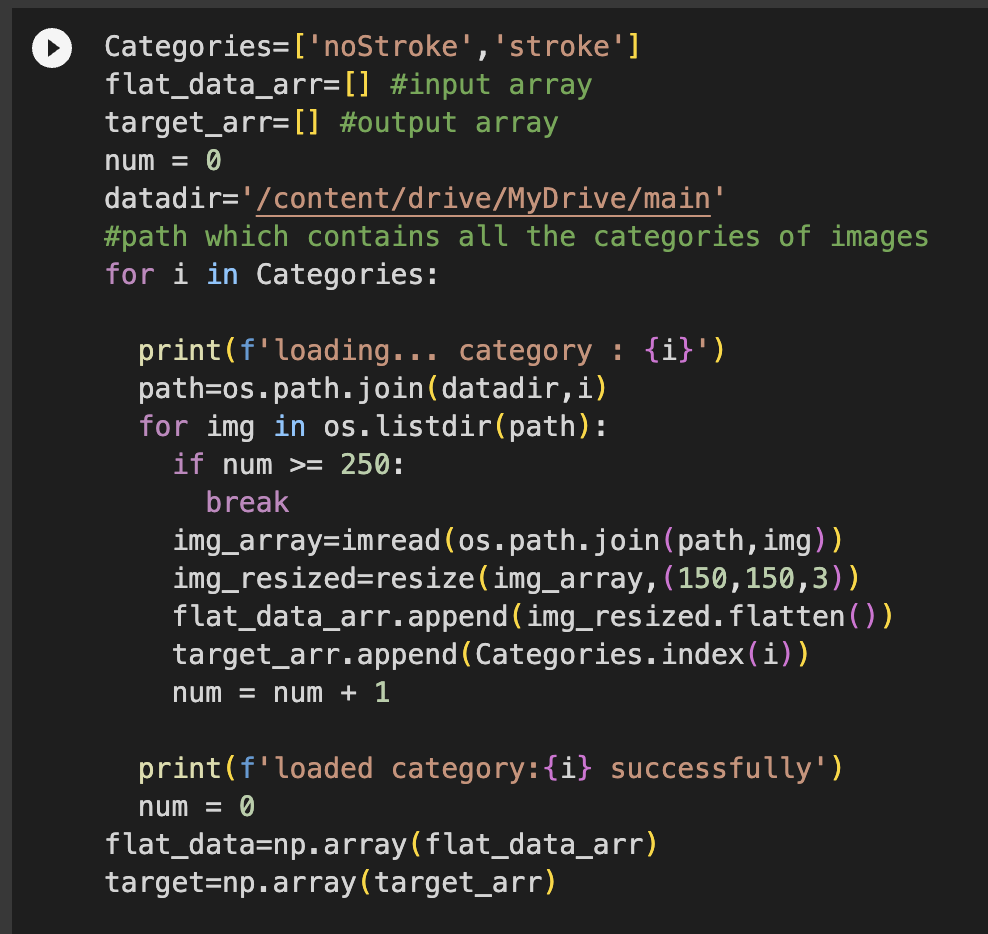
\includegraphics[width=8.5cm]{images/svm_data.png}
    \caption{Pre-processing data in Support Vector Machine}
    \label{fig:enter-label}
\end{figure}

% scikit-learn의 SVC를 불러와서 훈련을 진행했다. 훈련용 데이터와 테스트용 데이터는 위와 같이 각각 80%, 20%로 구성했으며 훈련 시간은 1시간 내외로 소요됐다.
Then, we loaded scikit-learn's SVC and ran training. The training time, which consists of 80\% training data and 20\% testing data, is approximately 1 hour.


% 테스트 검증 결과는 다음과 같다. 자세한 정확도를 구하기 위해 classification_report를 사용했고 모든 경우에서 88%의 정확도를 보였다. 하지만 테스트 데이터의 양이 50개로 매우 적어서 유의미한 결과라고 해석하기는 어려웠고, 학습도 어려움이 있어 여기서 다른 모델을 강구하기 시작했다.
The test verification results are as follows. We used classification\_report to obtain detailed accuracy and showed an accuracy of 88\% in all cases. However, the amount of test data was very small at 50, so it was difficult to interpret the results as meaningful, and learning was also difficult, so we started looking for a different model.

\begin{figure}[h]
    \centering
    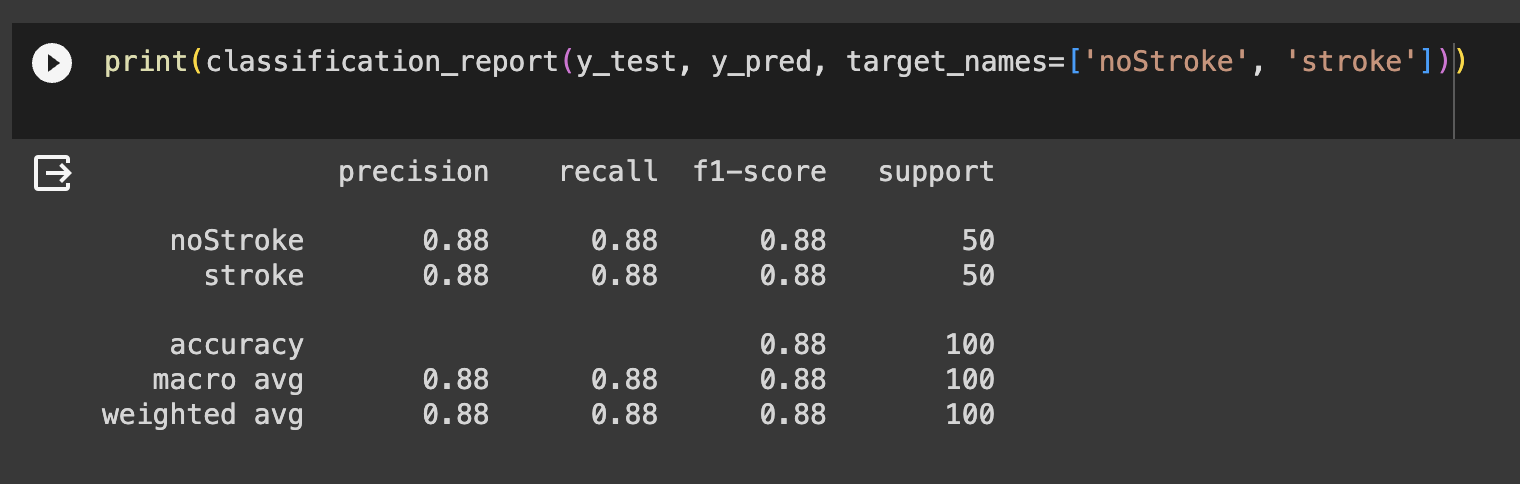
\includegraphics[width=8.5cm]{images/svm_result.png}
    \caption{The result of Support Vector Machine model}
    \label{fig:enter-label}
\end{figure}


% joblib 함수로 학습이 완료된 모델을 저장하고 AWS Lightsail로 옮겨 웹 서버로 배포했다. 이 때, 모델의 크기가 200MB를 넘었다. 이 점 또한 다른 모델을 찾아보기 시작한 이유 중 하나이다.
We saved the trained model using the joblib function, moved it to AWS Lightsail, and deployed it to a web server. At this time, the size of the model exceeded 200MB. This is also one of the reasons why I started looking for other models.

\begin{figure}[h]
    \centering
    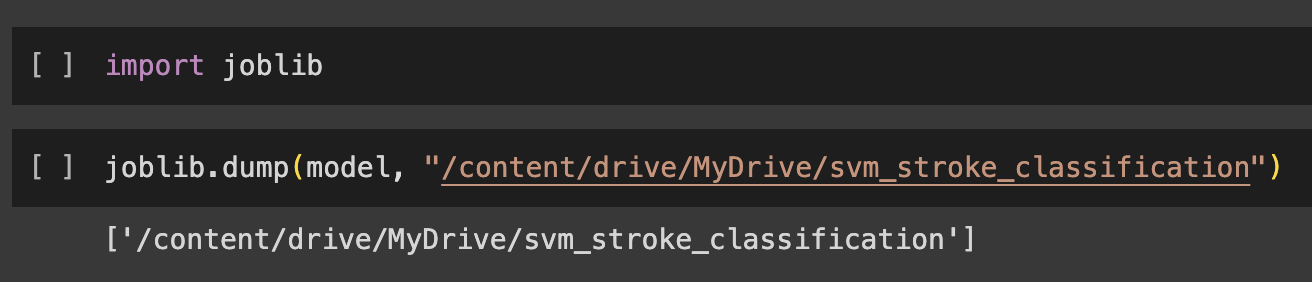
\includegraphics[width=8.5cm]{images/svm_save.png}
    \caption{Saving trained SVM model by using joblib}
    \label{fig:enter-label}
\end{figure}


\textbf{se\_svm.py} \\
% 위의 SE\_SVM.ipynb 파일을 python 파일 형식으로 저장한 것이다. 코드 파일의 내용은 위의 SE\_SVM.ipynb 와 같다.
The above SE\_SVM.ipynb file is saved in python file format. The contents of the code file are the same as SE\_SVM.ipynb above.


\textbf{SE\_ViT.ipynb} \\
% 이 파일은 ViT를 구현한 파일이다. ViT는 여러 모듈로 이루어진다. 이미지를 인식하기 위해 flatten시키는 patchify 모듈, patchify된 데이터에 원래 이미지에서의 위치 정보를 이식하는 positional_embedding 모듈, ViT에서 가장 중요한 작업인 Multi-head self attention을 수행하는 MSA 모듈, 이 모듈을 조립해 ViT class를 만들어서 구현을 완료한다. 
This file is a file that implements ViT. ViT consists of several modules. The patchify module that flattens the image for recognition, the positional\_embedding module that implants the positional information from the original image into the patchified data, and the MSA module that performs multi-head self attention, the most important task in ViT. These modules are assembled into a ViT class. Complete the implementation by creating.

% 학습에 필요한 데이터는 아래와 같이 전처리했다. pytorch 기반으로 ViT를 구현했으므로 Dataset과 이를 iteration할 수 있는 Dataloader를 직접 구현했다. 일관성을 유지하기 위해 흑백 사진으로 변환하고 이미지의 크기를 (150, 150)으로 바꾸었다. 사용한 함수는 다르지만 문맥은 위의 머신러닝 기반 모델과 동일하다.
The data needed for learning was preprocessed as follows. Since ViT was implemented based on pytorch, we directly implemented Dataset and Dataloader that can iterate on it. For consistency, I converted it to a black and white photo and resized the image to (150, 150). The functions used are different, but the context is the same as the machine learning-based model above.

\begin{figure}[h]
    \centering
    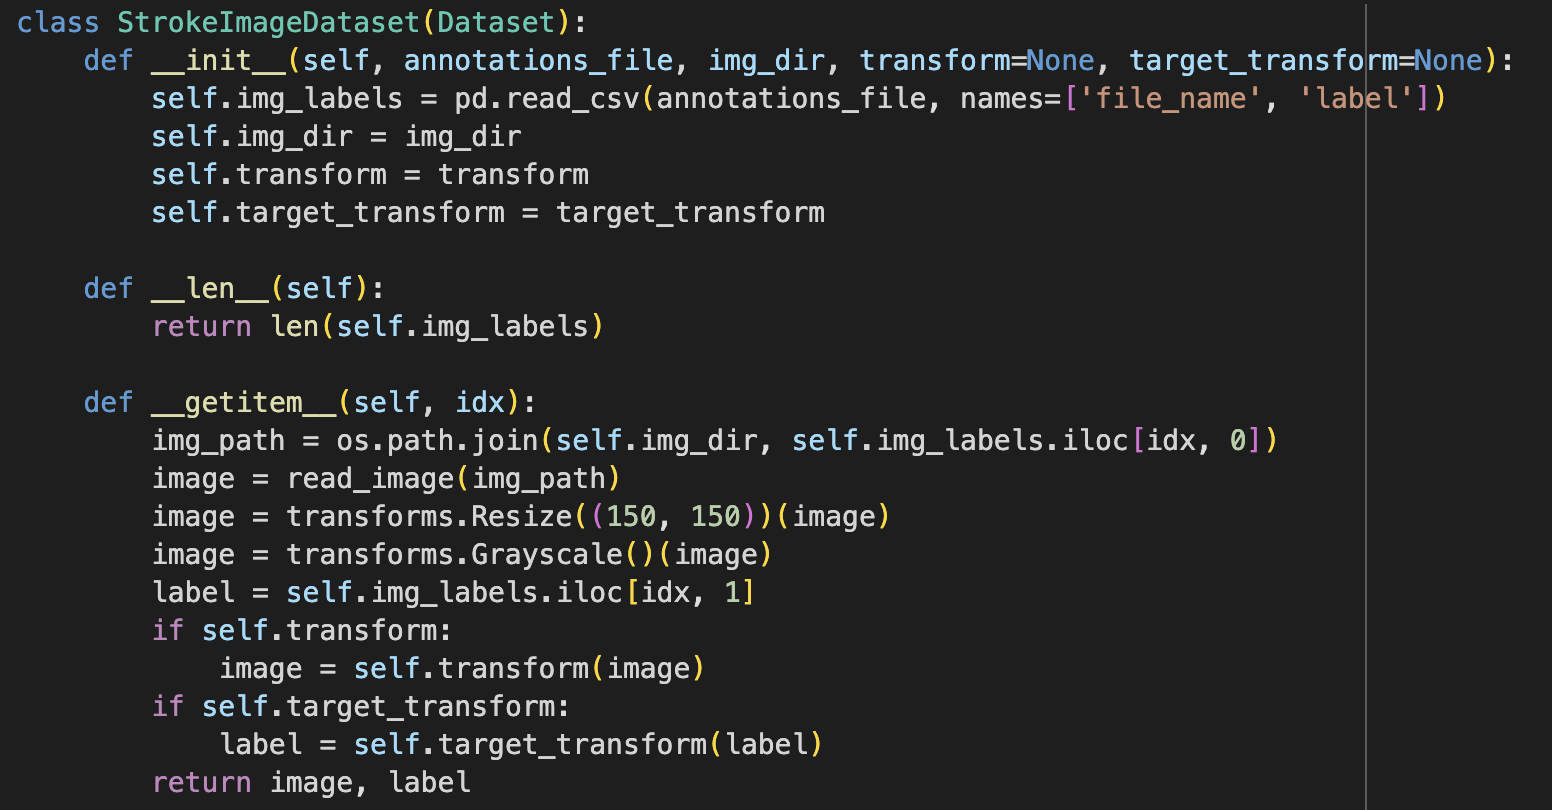
\includegraphics[width=8.5cm]{images/ViT_dataset.png}
    \caption{Dataset and Dataloader for ViT}
    \label{fig:enter-label}
\end{figure}

% 가장 중요한 MSA 모듈에 대해 상세한 구현은 다음과 같다. head 개수만큼 Q, K, V matrix를 pytorch의 Linear로 선언해서 back propagation으로 학습이 가능하도록 한다. 그리고 미리 주어진 입력에 대해 정해진 Q, K, V 내적을 진행해서 결과를 만들어낸다. 이 결과는 stack 형식으로 쌓여 있다가 모든 연산이 종료되면 입력과 동일한 차원으로 합병되어 출력한다. 즉, 연산 과정에는 head 개수만큼 분할되어 연산이 병렬적으로 진행된다. 
The detailed implementation of the most important MSA modules is as follows. Declare Q, K, and V matrices as Linear in pytorch as many as the number of heads to enable learning through back propagation. Then, the Q, K, and V dot products are performed on pre-given inputs to produce a result. These results are stacked in a stack format, and when all operations are completed, they are merged into the same dimension as the input and output. In other words, during the calculation process, the division is divided by the number of heads and the calculation is carried out in parallel.

\begin{figure}[h]
    \centering
    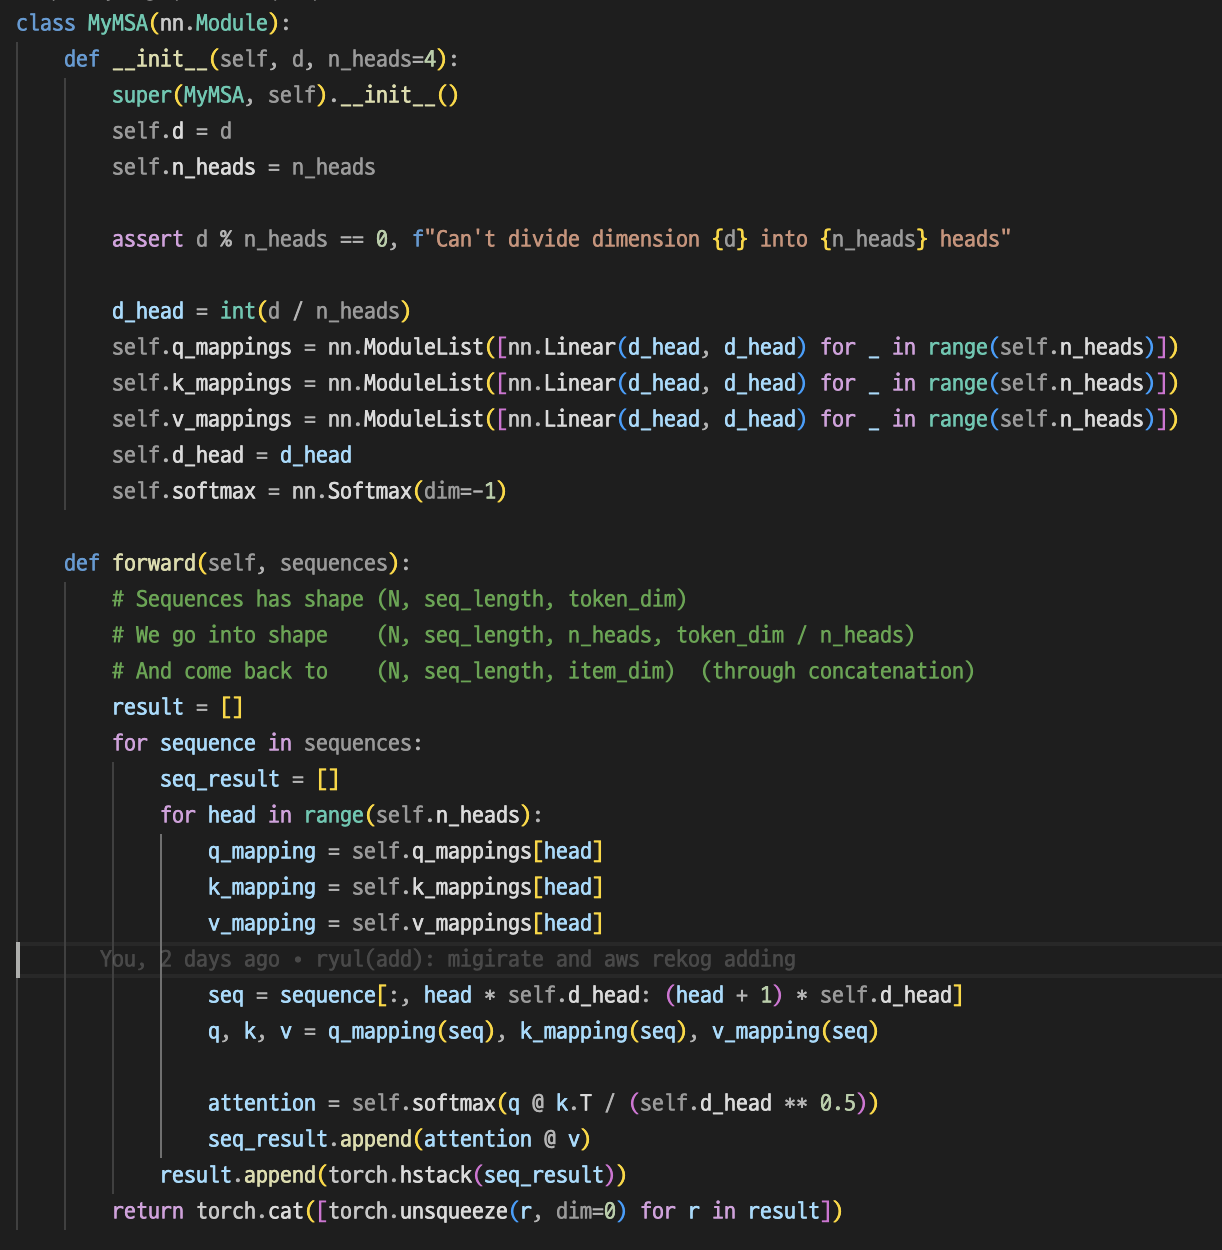
\includegraphics[width=8.5cm]{images/MyMSA.png}
    \caption{Implementation of Multi-head Self Attention}
    \label{fig:enter-label}
\end{figure}

% 위의 모듈을 만들고 아래 소스 코드와 같이 ViTBlock class를 만들어 이 class에 넣는다. 이 ViTBlock class는 MSA와 각종 결과의 정규화, Residual Connection이 포함된다.
After creating the above module, make a ViTBlock class as shown in the source code below, and insert it into this class. This ViTBlock class includes MSA, normalization of various results, and residual connection.

\begin{figure}[h]
    \centering
    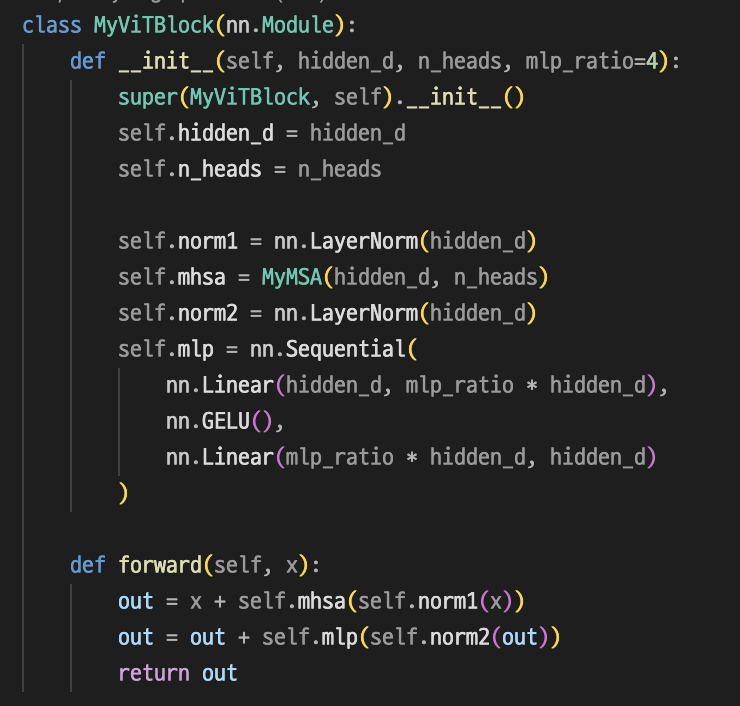
\includegraphics[width=8.5cm]{images/MyViTBlock.png}
    \caption{Implementation of ViTBlock}
    \label{fig:enter-label}
\end{figure}

% ViTBlock을 만들고 patchify, get_positional_embedding과 같은 데이터 전처리 과정을 포함해 최종적으로 아래와 같은 ViT class를 만들었다.
We created ViTBlock, including data preprocessing processes such as patchify and get\_positional\_embedding, and ultimately created the ViT class below.

\begin{figure}[h]
    \centering
    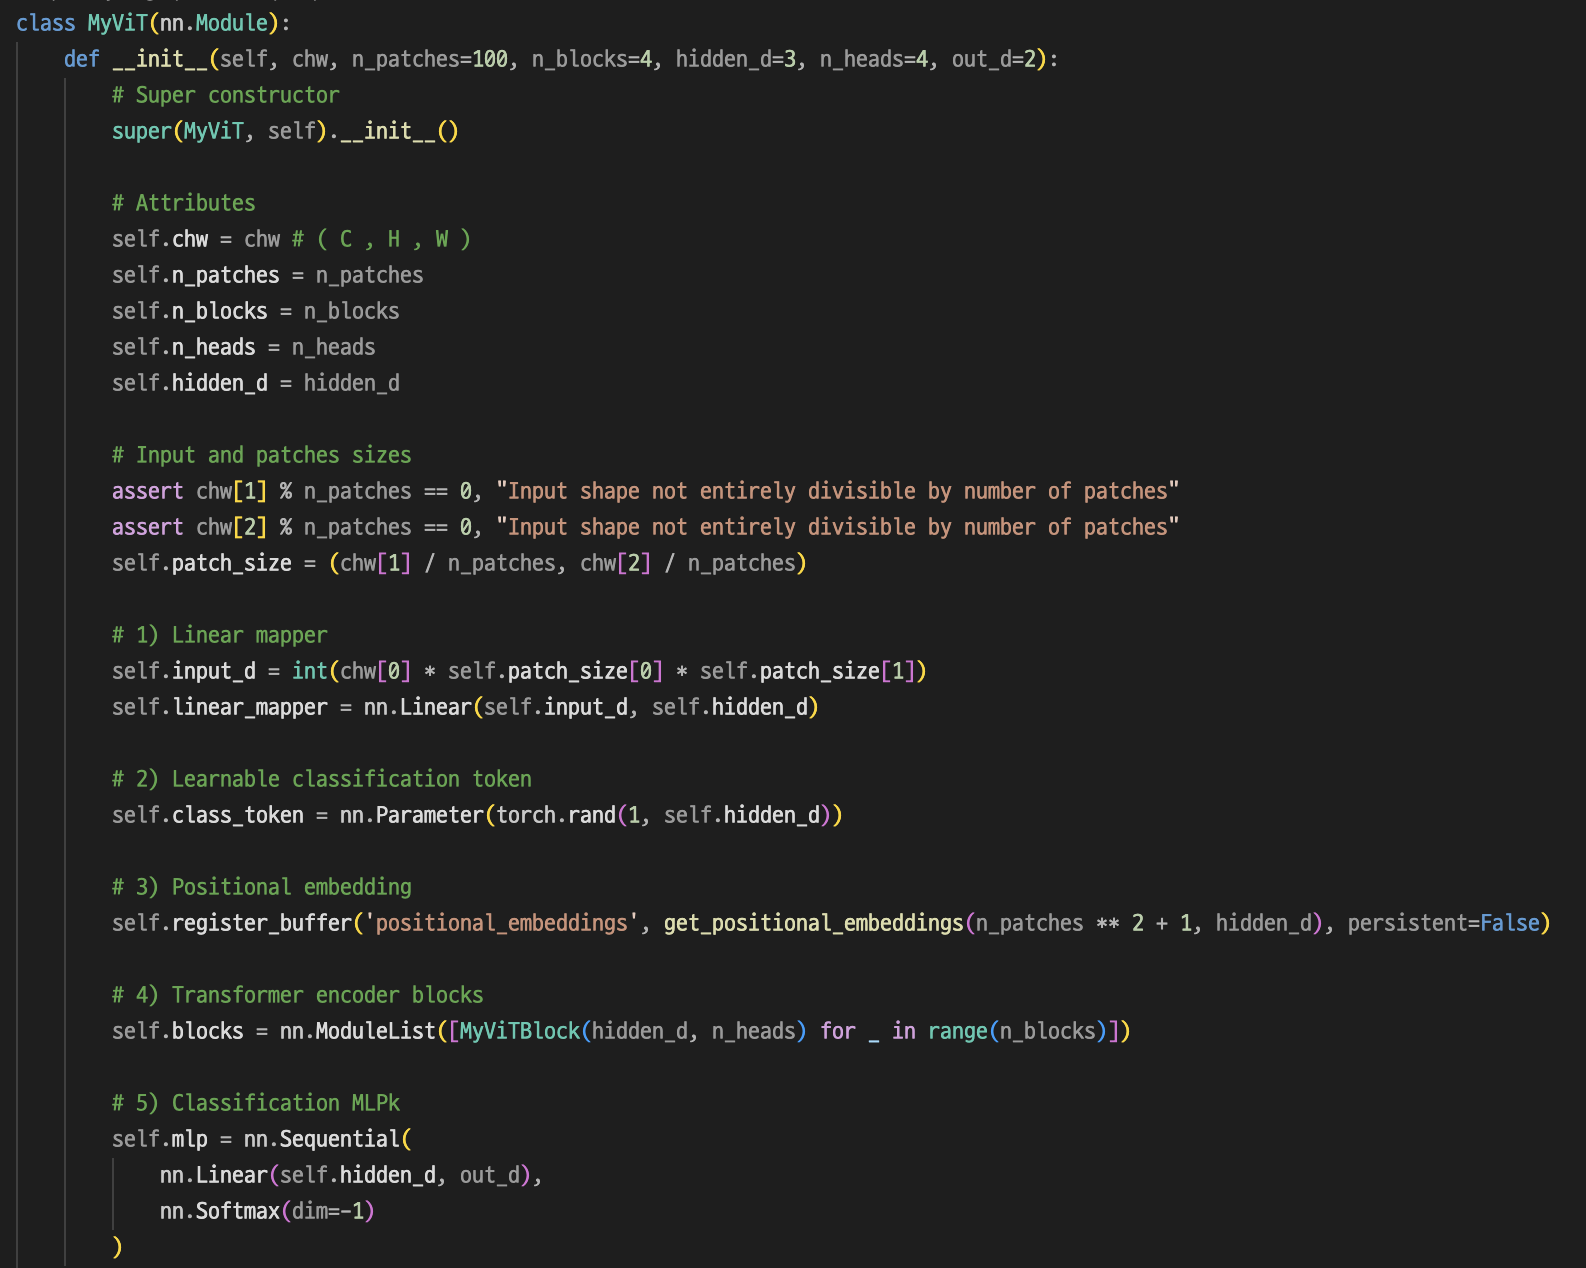
\includegraphics[width=8.5cm]{images/MyViT.png}
    \caption{Implementation of ViT class}
    \label{fig:enter-label}
\end{figure}

% 구현을 완료한 후에 main 문에서 테스트를 진행했다. Adam optimizer를 이용해서 5 epoch으로 훈련한 결과 66\% 정도의 정확도를 보였다. 수치 상으로는 제일 낮은 정확도를 보였다. 이는 학습이 충분히 이루어지지 않았다고 추론할 수 있다. ViT는 많은 데이터가 필요한데 환자의 의료 정보와 깊게 관련이 있어 충분한 양의 학습 데이터를 구하기 어려웠다. 또한 데이터가 augmented 된 데이터가 많아 중복된 데이터가 있다. ViT의 구조적인 문제와 현실의 상황 문제로 높은 성능을 나타내진 못한 것으로 생각된다.
After completing the implementation, testing was conducted in the main statement. As a result of training with 5 epochs using Adam optimizer, the accuracy was about 66\%. Numerically, it showed the lowest accuracy. This can be inferred that sufficient learning has not occurred. ViT requires a lot of data, but it is difficult to obtain a sufficient amount of learning data because it is deeply related to patients' medical information. Additionally, there is duplicated data as there is a lot of augmented data. It is believed that ViT did not achieve high performance due to structural problems and real-life situation problems.

\begin{figure}[h]
    \centering
    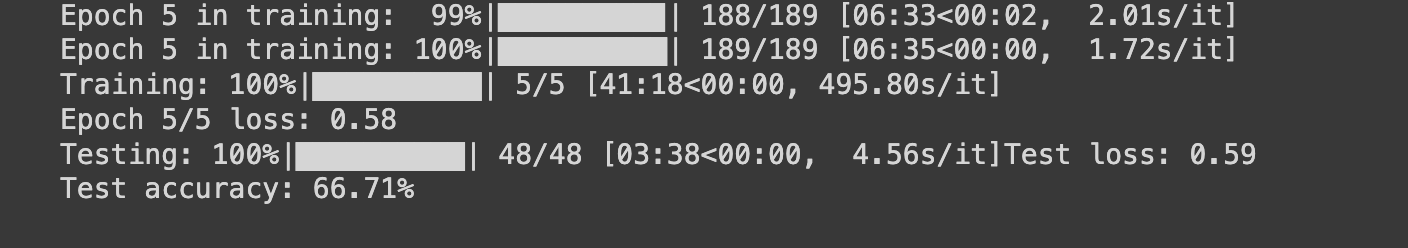
\includegraphics[width=8.5cm]{images/ViT_result.png}
    \caption{The result of testing ViT}
    \label{fig:enter-label}
\end{figure}

\textbf{se\_vitprac.py} \\
The above SE\_ViT.ipynb file was saved as a python file. The contents of the file are as above.

\begin{figure}[h]
    \centering
    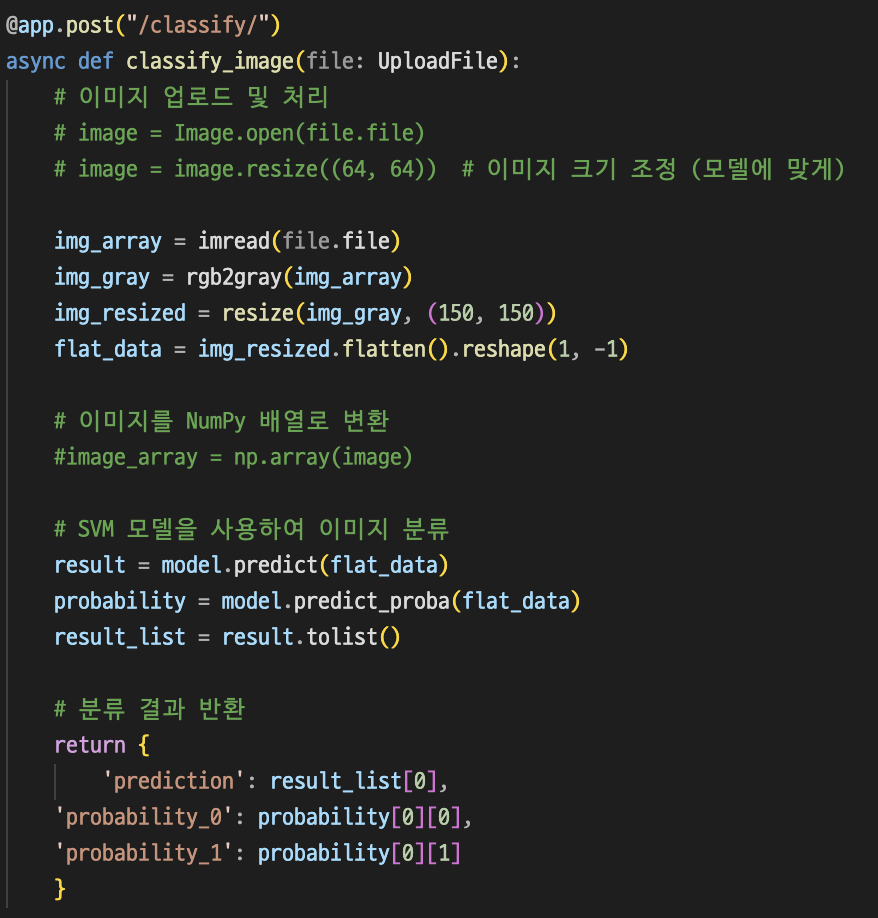
\includegraphics[width=8.5cm]{images/app.py.png}
    \caption{Core source code in app.py}
    \label{fig:enter-label}
\end{figure}

\textbf{app.py} \\
% 학습이 완료된 모델을 웹 서버로 배포하는데 사용되는 파이썬 파일이다. FastAPI와 uvicorn으로 웹 서버를 제작한다. annotation으로 @app.post("/classify/")를 붙여서 classify 형식으로 POST 요청이 왔을 때 함수가 실행되도록 만들었다. joblib 함수로 원하는 모델을 불러온다. 이미지 파일은 UploadFile의 file 변수로 받는다. 이 파일은 위 모델의 학습 과정에서 이미지 전처리 과정과 동일한 과정을 거친다. 이미지를 흑백으로 변환하고 사이즈를 통일시킨다. 그리고 벡터로 변환하고 이를 모델의 인자로 넘겨서 분류를 하도록 했다. 이때, 뇌졸중인지 아닌지 판단하고 각 상태의 확률을 함께 추론하도록 했다. 최종적으로 모델이 분류한 state와 각 state의 확률값을 json format으로 호출한 곳으로 넘겨준다. 
This is a Python file used to deploy the trained model to a web server. Build a web server with FastAPI and uvicorn. By adding @app.post("/classify/") as an annotation, I made the function run when a POST request came in classify format. Load the desired model with the joblib function. The image file is received as the file variable of UploadFile. This file goes through the same process as the image preprocessing process in the learning process of the model above. Convert the image to black and white and unify the size. Then, we converted it to a vector and passed it as a parameter to the model for classification. At this time, we were asked to determine whether it was a stroke or not and to infer the probability of each condition together. Finally, the state classified by the model and the probability value of each state are passed to the calling party in json format.

